\documentclass[12pt,a4paper]{article}

% ════════════════════════════════════════════════════════════════════════════
%  PACKAGES
% ════════════════════════════════════════════════════════════════════════════

\usepackage[utf8]{inputenc}
\usepackage[T1]{fontenc}
\usepackage{mathptmx}
\usepackage{microtype}
\usepackage{indentfirst}

\usepackage{geometry}
\geometry{
  left   = 1.5in,
  right  = 1.0in,
  top    = 1.5in,
  bottom = 1.5in,
  includefoot
}

\usepackage{graphicx}
\graphicspath{{../screenshots/}{./}}
\usepackage{hyperref}
\usepackage{xcolor}
\usepackage{verbatim}
\usepackage{textcomp}
\usepackage{amsmath}
\usepackage{amssymb}
\usepackage{booktabs}
\usepackage{longtable}
\usepackage{enumitem}
\usepackage{setspace}
\usepackage{tocloft}
\usepackage{abstract}
% datetime removed — use \today instead
\usepackage{caption}
\usepackage{float}
\usepackage{titlesec}

% ════════════════════════════════════════════════════════════════════════════
%  FORMAT SETTINGS
% ════════════════════════════════════════════════════════════════════════════

\doublespacing
\setlength{\parindent}{0.5in}
\setlength{\parskip}{0pt}
\raggedbottom
\emergencystretch=2em

\setlist[itemize]{
  leftmargin=0.65in,
  itemsep=2pt,
  topsep=4pt,
  parsep=0pt
}

\setlist[enumerate]{
  leftmargin=0.65in,
  itemsep=2pt,
  topsep=4pt,
  parsep=0pt
}

\captionsetup{
  font=normalsize,
  labelfont=bf,
  justification=centering
}

\hypersetup{
  colorlinks=false,
  pdfborder={0 0 0}
}

% ── Section = Chapter heading (display style, centred, all-caps title) ─────────
\titleformat{\section}[display]
  {\centering\bfseries\singlespacing\large}
  {CHAPTER \Roman{section}}
  {0.8cm}
  {\MakeUppercase}

\titlespacing{\section}{0pt}{0.5cm}{1.2cm}

% ── Subsection ─────────────────────────────────────────────────────────────────
\titleformat{\subsection}
  {\normalfont\bfseries}
  {\thesubsection}
  {0.8em}
  {}

% ── Subsubsection ──────────────────────────────────────────────────────────────
\titleformat{\subsubsection}
  {\normalfont\bfseries}
  {\thesubsubsection}
  {0.8em}
  {}

% ─────────────────────────────────────────────────────────────────────────────
\begin{document}

% ════════════════════════════════════════════════════════════════════════════
%  TITLE PAGE
% ════════════════════════════════════════════════════════════════════════════

\begin{titlepage}
  \centering
  \singlespacing
  \thispagestyle{empty}

  \vspace*{0.3cm}

  {\large\bfseries VIETNAM NATIONAL UNIVERSITY -- HO CHI MINH CITY\par}
  \vspace{0.25cm}
  {\large\bfseries INTERNATIONAL UNIVERSITY\par}
  \vspace{0.2cm}
  {\normalsize\bfseries School of Computer Science and Engineering\par}

  \vspace{0.6cm}

  \IfFileExists{Screenshot 2025-12-03 205743.png}{%
    \includegraphics[width=0.22\linewidth]{Screenshot 2025-12-03 205743.png}%
  }{%
    \fbox{\parbox[c][2.4cm][c]{2.4cm}{\centering IU Logo}}%
  }

  \vspace{0.6cm}

  {\Large\bfseries
    PATTERN-AWARE RETRIEVAL-AUGMENTED GENERATION OF\\[6pt]
    MULTIPLE-CHOICE QUESTIONS FROM LECTURE MATERIALS\\[6pt]
    USING LARGE LANGUAGE MODELS\par}

  \vspace{0.4cm}

  {\normalsize\itshape
    QuizGen: A Pattern-Aware RAG-Based MCQ Generation and Practice Platform\par}

  \vspace{0.8cm}

  {\normalsize By\par}
  \vspace{0.3cm}
  {\normalsize\bfseries Luong Quang Huy\par}
  \vspace{0.2cm}
  {\normalsize Student ID: ITITIU22076\par}

  \vspace{0.9cm}

  {\normalsize
    A thesis submitted to the School of Computer Science and Engineering\\
    in partial fulfillment of the requirements for the degree of\\
    Bachelor of Science in Computer Science\par}

  \vfill

  {\normalsize Ho Chi Minh City, Vietnam\par}
  \vspace{0.2cm}
  {\normalsize \the\year\par}
\end{titlepage}

% ════════════════════════════════════════════════════════════════════════════
%  FRONT MATTER
% ════════════════════════════════════════════════════════════════════════════

\pagenumbering{roman}
\setcounter{page}{1}

% ────────────────────────────────────────────────────────────────────────────
%  SIGNATURE PAGE
% ────────────────────────────────────────────────────────────────────────────

\newpage
\thispagestyle{empty}
\begin{center}
  \singlespacing

  {\bfseries
    PATTERN-AWARE RETRIEVAL-AUGMENTED GENERATION OF\\[6pt]
    MULTIPLE-CHOICE QUESTIONS FROM LECTURE MATERIALS\\[6pt]
    USING LARGE LANGUAGE MODELS\par}

  \vspace{2.2cm}

  APPROVED BY:

  \vspace{1.5cm}

  \makebox[4.2in]{\hrulefill}\\{}
  Dang Tam Nhan, Supervisor

  \vspace{1.3cm}

  \makebox[4.2in]{\hrulefill}\\{}
  Committee Member

  \vspace{1.3cm}

  \makebox[4.2in]{\hrulefill}\\{}
  Committee Member

  \vspace{1.8cm}

  THESIS COMMITTEE
\end{center}

% ────────────────────────────────────────────────────────────────────────────
%  ACKNOWLEDGMENTS
% ────────────────────────────────────────────────────────────────────────────

\newpage
\thispagestyle{empty}
\begin{center}
  \textbf{ACKNOWLEDGMENTS}
\end{center}

\vspace{1cm}

I would like to say thank you to my supervisor, \textbf{Dang Tam Nhan}, for showing me how to implement this project, as he has experience in evaluating and implementing RAG AI system. The monthly feedback helped me paved the way for not only building an app for generate MCQs questions but also show how to build a pipeline for collecting data, processing data and then making the MCQs with evaluation results. Those comments have helped me change and improved many parts of the thesis and how I build the project.

I also want to say thanks to the \textbf{Faculty of School of Computer Science and Engineering at
International University – Vietnam National University Ho Chi Minh City}. I have learnt many courses in the Network Engineer program that create my foundation of knowledge, especially Web App and Software Engineering


Huge thanks to my friends, especially \textbf{Dai Hoang Viet} and \textbf{Nguyen Phuc Dat} for helping with the early stress test and review, real users feedback for me to understand a stakeholder’s perspective for upgrading my app even more. The thesis will not be as good as this state if it does not have you guys’ help.

I say thank you to my family who has supported my study and gave me chances to enroll in university, never doubted me about my schooling thing.

Finally, I want to show gratitude to tools and communities that have me completed these prototypes and thesis, they are \textbf{FastAPI}, \textbf{Next.JS}, \textbf{LangChain}, \textbf{Groq}, \textbf{OpenRouter}, and \textbf{Google Gemini}. In this thesis, I used them for supporting the system, the pipeline but the design and idea implementation, setup remain my own responsibility.

\vspace{0.6cm}

\enlargethispage{2\baselineskip}

\begin{flushright}
\begin{minipage}{0.45\linewidth}
  \raggedleft
  \singlespacing
  \textit{Luong Quang Huy}\\[0.25cm]
  Ho Chi Minh City, May 6, 2026
\end{minipage}
\end{flushright}

% ────────────────────────────────────────────────────────────────────────────
%  TABLE OF CONTENTS / LIST OF TABLES / LIST OF FIGURES
% ────────────────────────────────────────────────────────────────────────────

\newpage
\tableofcontents

\newpage
\listoftables

\newpage
\listoffigures

% ────────────────────────────────────────────────────────────────────────────
%  ABSTRACT
% ────────────────────────────────────────────────────────────────────────────

\newpage
\begin{center}
  \textbf{ABSTRACT}
\end{center}

\vspace{1cm}

This thesis idea comes from my old habit when preparing for final exams for
some courses, specifically MCQ ones. I fed the test banks from previous
semesters into LLMs like ChatGPT, Grok, or maybe Google Gemini and then
asked them to copy or mimic the same patterns of how the lecturers create
questions, such as simple theory questions and applied ones. That workflow
is what I implemented, but it is too much manual work and too much
handholding while doing all those steps. One more problem is that the
materials, old question banks, and generated questions were kept in various
places and not in a unified place for easy management.

So, to solve those pains, I built QuizGen, a complete system that integrates
a pipeline for question analysis, generation, and review. It combines RAG,
exam-pattern conditioning, Bloom-level control, and a quiz practice flow. It
helps us to review for the upcoming topic for the exam, helps students
review them, and helps the lecturer shorten the time to create quality
quizzes. In the backend, we use semantic retrieval technique to get all the
context from the lectures, and few-shot conditioning to make sure that AI
will follow the old exam pattern.

In the app, I used Next.js for the front-end, FastAPI for the backend, and
SQLite for storing the data. PDFs, DOCX, and PPTX files are extracted and
split into word-level chunks of 2000 words with 200 words of overlap. The
chunks are then embedded and stored into the database. During the creating
phase, the system gets the source chunks with cosine similarity and places
them into the LLM prompt. The system has a grounding verification mechanism
to see if it is based on the lectures or not. It can also help students to
revise all the contents and prepare knowledge for exams, and they can also
check their history to see how good their results were.

Finally, after multiple evaluation runs with different AI models, the system
not only minimizes all the manual work but also demonstrates that it reduces
the time used for lecturers to create good and based quizzes. The students
also can achieve a better learning curve with the feedback loop.

\bigskip
\noindent\textbf{Keywords:} multiple-choice question generation,
retrieval-augmented generation, large language models, Bloom's taxonomy,
exam-pattern conditioning, educational technology.

% ════════════════════════════════════════════════════════════════════════════
%  MAIN TEXT
% ════════════════════════════════════════════════════════════════════════════

\newpage
\pagenumbering{arabic}
\setcounter{page}{1}
\section{Introduction}

\subsection{Background}

In these recent years of studying scenarios, collecting and storing old exam
banks is one of the most effective ways for seniors to pass down material to
junior students to optimize the learning path. With the appearance of LLMs
like ChatGPT and Gemini, it is also easier for them to use AI into creating
good quality revision tests, mimicking and analyzing the patterns. But this
process involves too many steps including repetitive prompting and continuous
handholding. One more downside is the generated contents, slides, lectures,
and patterns are fractured and are not unified in one place, so QuizGen was
born.

This personal experience highlights a practical approach to learning, not
only to understand but to make the learning curve more enjoyable. Students
can generate quick quizzes to refresh their brain, understand the pattern,
and understand keywords. Also joining with the exam pattern is better for
leveling their grades, not only to evaluate random ordinary questions but
also to follow how the lecturer asks the MCQs. Moreover, the lecturer can
use this system to relieve one of the major pain points, which is the quality
of the MCQs and the answers. The length of the answer will vary and
contribute to what makes a good exam paper.

In recent years, LLMs have actually gained that fast paced token output speed for text generation but if we use only raw text extraction and some basic filters, it will not be good enough for the actual exam revision, if there are no real strict constraints/ filters, the generated items are highly likely to drift outside the official syllabus.

Therefore, my objective is not only to use AI/LLMs to generate questions in
general, but to build a fully implemented system called QuizGen. It combines
RAG to follow the structure of the slides and lectures, a filtered system
that follows the exam pattern, and a review feature to evaluate the quizzes
generated by the app. So, it becomes a closed-loop system that can help
students and lecturers have better productivity.

\subsection{Motivating Scenario and Use Cases}

During traditional preparation for MCQ-based final exams, students often
face numerous manual steps, from accessing drive folders, asking senior
students to pass down exam banks, to switching to different tabs like LLMs,
Drives, Photos, and manually copy-pasting the prompt for LLMs. This makes it
highly difficult to focus on actual productivity and learning curve.
Moreover, the documents are very fragmented, making the process actually
cognitively overwhelming.

From the educators' perspective, a significant amount of time is continuously
spent on drafting weekly quizzes, crafting a clear question stem, one correct
answer, and three plausible distractors to ensure high-quality assessment
rather than superficial content. They also care a lot about privacy, not
wanting their lectures to be leaked on some unauthorized public platform.
They also need an agent for drafting all the quizzes to catch on with their
slides but can be modified before giving them to the end users, which are
students.

Students are rarely engaged by quizzes presented as raw text dumps on their
screens, which diminishes the realism of the testing experience. They need a
UI that has productive blocks that catch their attention, and the most
important part is that they need one with attempt history so that they can
see the progress they have made, to maintain learning motivation and monitor
their incremental progress. Moreover, both lecturers and students also want
empirical proof of content grounding, specifically identifying the exact
lecture pages used by the LLM to generate those questions, thereby
mitigating hallucination risks.

To bridge these interconnected gaps, QuizGen was developed as a complete
closed-loop system that supports both students and lecturers, combining all
processes into one fully functional web application. First, lecturers upload
their contents, such as slides, PDFs, DOCX files, or PPTX files. Then they
can choose the right exam pattern, such as midterm or final, and check the
grounding of the questions generated by LLMs before proceeding to publish
the exam. End users like students can begin to practice the exam question
set, receive the final results instantly after finishing it, and watch the
dashboard for better topic clarification or Bloom-level analysis, showing the
interactive feedback loop.

\subsection{Problem Statement}

From the perspective of a lecturer in managing their resources, this is a
very common problem. Lecturers are good with what they are teaching and they
have the knowledge, but creating a good MCQ set is another story, which is
very time-consuming. One lecturer has so many layers and many chapters. The
work of typing each MCQ, with a stem, one true answer, and three distractors
week by week will cause a bottleneck in productivity. Humans who produce
high-quality exams cannot avoid facing cognitive fatigue.

The most dangerous part of using an LLM to generate MCQ questions is that AI
can be prone to hallucination. In reality, LLMs are very good at generating
structured passages, but with raw prompting, the chances of hallucination are
likely to appear. The questions may sound very general and very based on the
lectures, but sometimes it will likely be out-of-syllabus content. Students
who learn from these unverified mock exams may be drifted away from what is
actually there in the pattern or in the exam. The absence of factual
anchoring based on the actual lecture slides represents a major gap in raw
LLM utilization.

At International University specifically and other universities in general,
there exists a distinct stylistic fingerprint for each lecturer. Some want
code-analyzing problems, some like calculation a lot, and others like
theoretical questions. Raw LLMs, if not provided with enough context using
few-shot conditioning, always output the easiest level of Bloom Taxonomy,
which is Remember. This explains the occurrence of cognitive level
misalignment.

\subsection{Scope and Objectives}

The most important factor when designing this web application and designing
the pipeline was that I always wanted to focus on the downside of manual
work, why it is time-consuming, why it is too tiring to work like that, and
then focus on the objective. I want students and lecturers to really use the
system and to have a fully functional system that stores all the slides,
lectures, histories, and progressions to catch up with their learning curve
path, and also to centralize all the fragmented pieces.

The system has a structured pipeline that is fully integrated into it, from
uploading to reviewing the quizzes. It begins with preprocessing the
lectures, slides, PDFs, DOCX files, and PPTX files. The RAG aspect is used
to look up the context before giving the LLM those chunks, instead of only
using the base knowledge of the LLM. Filtering through few-shot conditioning
controls the difficulty level and also the structure of MCQs. The generated
data is packaged into a predefined JSON format, including the stem, options,
correct answer, explanation, and Bloom labels. Source checking is used for
grounding checks to support, but not to replace, human checking. This helps
lecturers define which questions are not based on the slides, lectures, or
contents. The interactive loop connects the whole pipeline from generation
to actually doing quizzes, with timer, history, and dashboard functions also
included. The system is also evaluated with many eval runs to test the golden
data and compare the results with each loadout of styles.

Although the system uses many techniques and a modern tech stack, it still
has many flaws and limits. It is not a production-ready, high-concurrency
platform. It uses only a SQLite database and calls AI APIs, and the localhost
running server mainly serves the academic purpose only. The datasets are
only basic English and Vietnamese. To make sure academic integrity is still
there, QuizGen only serves as a support and drafting tool, and it cannot
replace lecturer review. The grounding score also does not make sure that
100\% of generated questions are good. Rolling out this system without more
testing will not be fully supported.

\subsection{Research Questions}

This thesis was followed through three main questions I personally asked:
how was the performance, how were the results, and whether the whole
implemented workflow was valid enough. RQ1 focuses on the grounding efficacy
of RAG, examining whether its integration increases the factual anchoring of
the MCQs generated by LLMs, directly evaluating results against raw
prompting. This checks if it is really helpful to make AI know more context
than only using its own pre-trained knowledge.

Moving on to the second question, RQ2 asks about the validity of using
exam-pattern conditioning and few-shot pattern conditioning with an
instructed and distributed predefined Bloom level. The purpose is to see
whether this can make the AI generate higher levels of Bloom Taxonomy, such
as Apply and Analyze, without using fine-tuned models.

The final question is about the web application applied with the pipeline:
whether it can be a smooth interaction experience for end users, from upload,
creating, reviewing, to the dashboard function, and whether the closed-loop
implementation is valid enough.

All of those questions have already been answered inside the thesis. There
are full answers and partial answers, but they make clearer goals for future
development and act as a solid base and foundation for the future. For the
first question, I used semantic grounding score and a verifier, which is
another LLM called to check the results. RQ2 is quantitatively measured via
Bloom KL divergence and failure analysis. Finally, the web-application part
is tested by smoke tests, manual web workflow testing by human, and API
endpoint execution.

\subsection{Assumptions and Proposed Solution}

In this version, I did not design QuizGen for every possible classroom
situation. It needs input lectures, slides, or contents uploaded into the
pipeline. If the lecture file is not complete or is poorly extracted, the
generated questions will also be less reliable. I also encourage every end
user to review all the content created by this system before using it for
any formal assessment. For this reason, QuizGen is treated as a drafting and
practice tool, not an automatic exam-creating tool.

QuizGen is my proposed idea for turning my manual process into a fully
closed-loop system for lecturers and students to practice. Instead of raw
prompting with an LLM and a high risk of hallucination, the system gives the
model retrieved lecture content, optional exam pattern, and Bloom-level
instructions. The goal is not only to generate quizzes faster, but also to
help students more easily trace and review their knowledge based on their
needs.

The app begins when the end user uploads a file, which can be PDF, DOCX, or
PPTX based on their needs. The backend extracts the text and divides it into
overlapping chunks so that important contents or examples are less likely to
be lost at chunk boundaries. These chunks are embedded and stored for later
retrieval. When the user requests a quiz, it searches for the chunks that
are most relevant to the selected topic and places them into the prompt as
source context. If a pattern is selected, the prompt also includes
sample-question style and target difficulty information. In the end, after
all those filters, generated content follows both the lectures and the exam
format pattern.

Those generated questions always have the same format, with metadata inside
it, including four answer options, answer key, difficulty tag, and Bloom
label. The grounding evaluator helps users see if the question is close to
the uploaded source material, but it does not prove that the questions are
perfect.

\subsection{Thesis Structure}

This thesis has six chapters in total. Chapter I is about the background,
motivation, problems stated in the thesis, the questions, and the proposed
solution. Chapter II is about the foundations of this pipeline, how things
work, the state of LLMs in education, what RAG is, how I use prompting,
Bloom's Taxonomy, and existing question generation tools on the market.
Moving on to Chapter III, it explains how I designed the system and the
pipeline, where end users begin with uploading documents, retrieving
contents, recognizing patterns, generating MCQs, and then grounding with
evaluations. Chapter IV describes how I implemented everything from scratch,
including backend, frontend, dataflow, API workflow, quiz practice, and all
the testing evidence for the thesis. Chapter V is one of the most important
parts of the thesis, where I show the evaluation data, results of runs, and
discuss the failure cases. I close the thesis with Chapter VI, where I
summarize what I built, what is there in the evaluation, and what gaps are
still there.

\begin{figure}[H]
  \centering
  \singlespacing
  \fbox{%
    \begin{minipage}{0.80\linewidth}
      \centering
      \vspace{0.3cm}
      Chapter I: Introduction\\[6pt]
      $\downarrow$\\[6pt]
      Chapter II: Literature Review\\[6pt]
      $\downarrow$\\[6pt]
      Chapter III: Methodology and System Design\\[6pt]
      $\downarrow$\\[6pt]
      Chapter IV: Implementation and Results\\[6pt]
      $\downarrow$\\[6pt]
      Chapter V: Discussion and Evaluation\\[6pt]
      $\downarrow$\\[6pt]
      Chapter VI: Conclusion and Future Work\\[0.3cm]
    \end{minipage}%
  }
  \caption{Structure of the thesis.}
  \label{fig:thesis-structure}
\end{figure}

\clearpage
\section{Literature Review}

\subsection{Large Language Models in Education}

I review LLMs in education because my system uses LLMs to produce the
questions, acting as a question writer, but not as the whole integrated
pipeline. The survey of Xu et al.\ \cite{xu2024survey1,xu2024survey2} helped
me understand that AI or LLMs can help students and lecturers in adaptive
learning and assessment. But after the research, I found out that the
problem is not about how strong the LLM is. In academic use in general,
fluent text generation is not enough, because it still needs human
evaluation and review.

In my research, I saw that many education systems use LLMs just to answer
questions or maybe explain the contents. This can work, but it is too broad
and does not have enough filters. Because of that, I built QuizGen to focus
on one pipeline process: based on lecturer material, generating MCQs, helping
students review them, and practicing with them. The implemented workflow
focuses on a closed-loop system more than just an LLM interface.

We can see that ChatGPT-based tools can support learning by answering
questions, giving ideas, or maybe solving an entire problem
\cite{frontiers2024chatgpt}. In the research of Pham et al.\
\cite{ieeebigdata2023}, prompt engineering can generate many questions from
a passage. But moving into my pipeline, raw prompting is not good enough
because the system implements retrieved chunks, validation, and lecturer
review. In the real case of my thesis, the prompt is just the beginning of a
pipeline, the kick start of many processes before and after that.

LLMs are very strong, and that is one fact we cannot deny. But one thing
proved in the research by Danyaro et al.\ \cite{danyaro2024hallucination} is
that hallucination is the cause of many AI failures. The content generated by
LLMs can sound very precise and smooth. In the quiz system, AI cannot make
mistakes too freely, because hallucination makes the AI sometimes not realize
what it is doing, leading to failures. Because of that, this pipeline needs
retrieval and grounding signals for filtering to improve the content
generated by it.

There are also more systems showing that AI is being integrated and used a
lot in other systems, like intelligent tutoring systems
\cite{anderson1985its} that focus on learner state and feedback systems.
Khanmigo \cite{khanmigo2026} and Duolingo Max \cite{duolingo2023max} show
that AI is being placed in the position of a product or workflow in
studying. From that, QuizGen's implementation should be used in the learning
workflow, not just generated out for end users as an output. After being
generated, it should move into attempt, review, score, and dashboard.

Project Essay Grade \cite{springer2022aes} shows one more thing:
educational AI should not be evaluated only by fluency. With QuizGen,
grounding check is essential, along with Bloom alignment, answer correctness
signals, and workflow coverage in the whole system. Automated essay scoring
is useful, but while building QuizGen I had one thing in mind: any AI content
generated should always be reviewed by more criteria.

\subsection{Retrieval-Augmented Generation}

RAG is used to make the LLM look at the provided lectures first before
creating any content. In the research of Lewis et al.\ \cite{lewis2020rag},
RAG retrieves passages and then puts them into the generator, but in my
project, there are differences in how I use RAG to actually help improve the
system. It is not some Wikipedia store or big document collection. Uploaded
lectures are split and stored into chunks. So from what we know, RAG
implemented here is not for building a large search engine but to take the
right information from the lectures.

LLMs can generate MCQs that sound right, but the content may still be
outside of the lectures provided. With MCQ practice, the risk is that
students actually study the thing that is not from their lectures. In
technical terms, RAG helps put the relevant chunks close to the requested
topic inside the prompt, so that the model has fewer reasons to base on
general knowledge. But this also does not guarantee that the result will be
automatically correct.

About RAGAS \cite{es2023ragas}, I do not use it like a library or a full
framework, but it affected my way of thinking about evaluation, not the exact
implementation. RAGAS divides retrieval quality and generation faithfulness.
In QuizGen, I also divide the metrics: retrieval metrics, semantic grounding
proxy, judge score, and Bloom alignment. In my implementation, a good
retrieval method does not equate to a good question set, and good questions
do not automatically mean they are grounded.

In passage retrieval technique, BM25 \cite{robertson2009bm25} is very strong
with queries that have strong keywords, because it increases based on the
repetition of words. On the other hand, Dense Passage Retrieval
\cite{karpukhin2020dpr} is stronger when the query paraphrases the content
again. So with this system, lecture materials often come in many slides and
PDFs, and dense embeddings are more precise here. If I used exact keywords
only, it would not be stable and the grounding semantic percentage would be
lower.

In this thesis, I also tested Hybrid search and reranking through Reciprocal
Rank Fusion \cite{cormack2009rrf} and neural reranking
\cite{nogueira2019bert}, but to be sure, the results are not always too
good. I implemented them with a mindset to improve the quality of the
pipeline, but the evaluation results were not stable enough. It may have
potential, but in this small design idea, it is not stable enough yet.

Moreover, I researched that FiD \cite{izacard2021fid} and REPLUG
\cite{shi2023replug} are advanced methods of RAG, but in the scope of
QuizGen, they are not suitable. Both FiD and REPLUG show that they can
connect retrieval and generation deeper, but QuizGen is running by hosted
LLM APIs. I do not interfere too deep inside the model architecture, so I use
retrieved chunks, put them into a prompt, generate structured JSON, and
evaluate the result.

RAG is what makes the LLM understand the context of the lectures inputted
into the system, not to make sure the generated content is always correct.
It can take the right topic but not the best evidence to evaluate that.
Models can also read the correct chunks but choose the wrong answer key. So
in this state, I want to show that retrieval is only the first step of the
pipeline, not the real quality guarantee.

In some early tests, the errors or bugs were not always obvious. Some are
obvious ones but some are just hiding inside the technical view. There are
MCQs that are in the right topic but generate a lot more details that are
not inside the lectures. From that, I decided to keep the grounding score
based on percentage and I did not treat RAG as the complete solution for my
pipeline.

\subsection{Prompt Engineering and Few-Shot Learning}

One main design of QuizGen is that it uses hosted LLM APIs and not
fine-tuned models. Because of that, everything used to control the input,
output, and filters needs to be inside the prompt. I need to make the prompt
clear enough so that LLMs in general can understand the task. The prompt has
to include source material from retrieved chunks, exam pattern, difficulty
distribution, Bloom instruction, and a JSON structured schema.

Before researching deeper, I mostly used raw prompting with some constraints
and filters. I used roles, schema, and examples to get the output like I
wanted. The research of White et al.\ \cite{white2023prompt} helped me
understand deeper that every part of a prompt needs to be clear, not only
persona, template, or few-shot examples. Persona in the prompt helps the LLM
act like an experienced lecturer. Template helps structure the output.
Few-shot examples show the model what the exam pattern looks like. In
QuizGen, these outputs need to be precise because the backend needs to parse,
store, review, and then display generated questions.

In my own study habit and exam preparation, the first thing I look up is the
old exam banks passed down from seniors. From those old questions, I can
learn how long the questions are, what types are there, and how lecturers
put distractors inside the MCQs. From that idea, this approach helped me
build what the system looks like right now. QuizGen uses few-shot learning
\cite{brown2020gpt3} by putting sample questions inside the prompt to guide
the style, option format, difficulty, and most importantly Bloom's level.

From the papers I researched about chain-of-thought and self-consistency
\cite{wei2022cot,wang2022selfconsistency}, I understood better that long
prompts with clear structure give models more chance to process complex
MCQs. Because of that, application and analysis questions need better
instructions than only a simple ``generate quizzes'' command. However,
QuizGen does not show long reasoning text to students. I keep the final
output clean because clean output is one part of the user experience and it
also helps the backend parser.

When I first tested the application, LLM output did not always follow the
structure I wanted. Sometimes the model added unnecessary explanation that
was not in the prompt. Sometimes it lost fields, and sometimes the format
could not be parsed. Because of that, I made the prompt stricter so the
backend can validate and store questions more easily. This design does not
guarantee smooth and natural MCQs, but it makes the pipeline stable from
generation to review and quiz practice.

\subsection{Bloom's Taxonomy and MCQ Quality Control}
\label{subsec:bloom}

In the early testing phase, I saw that models generally generated
definition-style questions when the prompt did not state the Bloom level and
the type of questions. This made the generated contents look less aligned
with the lecture and less useful for real exam revision. Bloom's taxonomy
\cite{bloom1956taxonomy} and the revised taxonomy by Anderson and Krathwohl
\cite{anderson2001taxonomy} give the system a practical way to describe
cognitive level, such as remember, understand, apply, and analyze.

From the research of Pan et al.\ \cite{pan2019nqg}, I acknowledged that
automatic question generation systems often follow lower-order questions. In
QuizGen, Bloom is not just a label for better UI or UX. I use Bloom for two
main purposes. First, I use it to guide the model to create questions based
on the cognitive level that I really want. Second, I use it to evaluate the
generated distribution through Bloom KL divergence, so Chapter~V can compare
the requested Bloom distribution with the generated Bloom distribution.

Although Bloom helps control the cognitive level of questions, MCQ quality
also depends on a clear answer key, suitable distractors, explanation related
to the lecture, and source support for grounding. Kurdi et al.\
\cite{kurdi2020aqg} helped me understand that automatic question generation
is not only about generating a question sentence. It also needs educational
validity. Because of that, QuizGen does not treat Bloom as the only quality
signal.

In the end, Bloom's level is still metadata created by the model. It has no
academic authorization percentage by itself. Inside the backend, the system
checks that the label is inside the allowed values, and the evaluation checks
the system-level distribution. Lecturers still need to review the generated
questions because Bloom alignment cannot prove that the answer key is
correct, the distractors are suitable, or the source support is strong
enough.

\subsection{Existing Question Generation Systems and Tools}

A 2025 IEEE review of transformer- and LLM-based MCQ generation
\cite{ieee2025mcqsurvey} shows that most systems use either fine-tuning or
prompt engineering. This helped me position QuizGen: I do not fine-tune a
model, but I also do not rely on a single prompt. I combine prompt
engineering with retrieval, pattern examples, and a practice interface.

E-QGen \cite{eqgen2024} shows that structuring the prompt around role,
task, context, and format improves question generation quality. However, it does not provide
the same grounding workflow used in QuizGen. The BUE AQG System
\cite{bueaqg2024} combines keyword extraction and generation, and it reports
lecturer satisfaction, but it does not include exam-pattern conditioning or
student attempt tracking. The COLING 2025 work \cite{coling2025mcq} also
shows that prompting can generate MCQs from documents, but its output is not
connected to a full practice workflow.

Commercial tools show the practical demand for this kind of system. GPT Quiz
Generator, Quillionz \cite{quillionz2026}, and Questgen
\cite{questgen2026} focus on helping users create quizzes quickly. They are
useful comparisons because they show that teachers want productivity tools.
However, their public descriptions do not show the same combination that I
evaluate in this thesis: lecture retrieval, exam-pattern conditioning, Bloom
KL measurement, grounding status, and student practice analytics.

Generic ChatGPT prompting is also included as the simplest baseline. It is
close to the manual workflow I used as a student: paste material, paste
examples, and ask for more questions. This baseline is important because it
shows what is gained when the same idea is moved into a structured system.

Table~\ref{tab:system-comparison} summarises the key features of these
systems relative to QuizGen.

\begin{table}[H]
  \centering
  \singlespacing
  \caption{Comparison of existing question generation systems and QuizGen.}
  \label{tab:system-comparison}
  \begin{tabular}{@{}lccccc@{}}
    \toprule
    \textbf{System} &
    \textbf{\shortstack{Source\\grounding}} &
    \textbf{\shortstack{Exam\\pattern}} &
    \textbf{\shortstack{Bloom\\control}} &
    \textbf{\shortstack{Quiz\\practice}} &
    \textbf{\shortstack{Performance\\analytics}} \\
    \midrule
    Generic ChatGPT prompting  & \texttimes & \texttimes & \texttimes & \texttimes & \texttimes \\
    GPT Quiz Generator (Forms) & \texttimes & \texttimes & \texttimes & \texttimes & \texttimes \\
    E-QGen \cite{eqgen2024}    & \texttimes & Partial    & \texttimes & \texttimes & \texttimes \\
    BUE AQG \cite{bueaqg2024}  & \texttimes & \texttimes & \texttimes & \texttimes & \texttimes \\
    COLING 2025 \cite{coling2025mcq} & \texttimes & \texttimes & \texttimes & \texttimes & \texttimes \\
    Quillionz \cite{quillionz2026} & Partial & \texttimes & Partial & \texttimes & \texttimes \\
    Questgen \cite{questgen2026}   & Partial & \texttimes & \checkmark & Partial & \texttimes \\
    \textbf{QuizGen (this thesis)} & \checkmark & \checkmark & \checkmark & \checkmark & \checkmark \\
    \bottomrule
  \end{tabular}
\end{table}

\subsection{Evaluation Approaches for Generated Questions}

I evaluate QuizGen with several signals because one score is not enough for
MCQ generation. A question can be fluent but unsupported, grounded but too
simple, or aligned with Bloom level but have a weak distractor. These cases
need different checks.

BLEU and ROUGE are not the main metrics here. They compare generated text
with reference text, but there are many valid ways to ask a question from
the same lecture paragraph. I use task-specific metrics instead.

Retrieval is checked with Recall@$k$ and MRR. Grounding is checked with a
normalized cosine similarity proxy. Bloom alignment is checked with KL
divergence between the requested and generated Bloom distributions. Overall
question quality is estimated with an LLM judge rubric. In the post-review
ablation, I also add topic confusion and machine answer correctness to catch
failures that the first metrics do not show clearly.

The setup is limited in scope but sufficient for isolating whether
improvement comes from retrieval, from pattern conditioning, or from
model output quality.

\subsection{Research Gap}

Reading the literature and trying some of the existing tools revealed four
things that were missing from what I needed.

First, no tool I found gave a grounding signal that was directly tied to the
uploaded lecture file. Questions can be generated from a broad prompt, but
the student has no way to know whether a question actually tests the right
material. Second, existing tools do not use past exam questions as a style
reference. When I used ChatGPT manually, I had to paste old questions and
hope the model noticed the pattern. Nothing in the literature automates
that step in a usable way. Third, most tools mention difficulty, but none I
found checked whether the generated question set follows a specific Bloom
distribution. The label is attached, but not verified. Fourth, generating a
list of questions is only part of the task. None of the tools connect the
generated questions to a practice workflow where attempts, explanations,
history, and progress are stored.

QuizGen was designed to fill all four gaps at once. This is the main
difference between this prototype and a standalone question generator: the
pipeline does not stop at generation, and every design choice was driven by
one of those missing pieces.

\clearpage
\section{Methodology and System Design}

\subsection{Proposed Framework Overview}

QuizGen is designed as a nine-stage pipeline. This design came from the
limitations I saw when using a normal chat prompt for self-practice. A
single prompt can produce questions, but it does not remember documents,
does not manage old patterns, does not validate JSON output, and does not
store practice attempts. I separated the work into document ingestion,
retrieval, generation, review, and quiz practice.
Figure~\ref{fig:framework} illustrates the complete workflow.

\begin{figure}[H]
  \centering
  \singlespacing
  \fbox{%
    \begin{minipage}{0.82\linewidth}
      \centering
      \vspace{0.3cm}
      \textbf{Stage 1:} User uploads PDF / DOCX / PPTX\\[4pt]
      $\downarrow$\\[4pt]
      \textbf{Stage 2:} Text extraction and overlapping chunking\\[4pt]
      $\downarrow$\\[4pt]
      \textbf{Stage 3:} Chunk embedding via configured embedding provider\\[4pt]
      $\downarrow$\\[4pt]
      \textbf{Stage 4:} Semantic retrieval of top-$k$ relevant chunks\\[4pt]
      $\downarrow$\\[4pt]
      \textbf{Stage 5:} Optional exam-pattern injection into prompt\\[4pt]
      $\downarrow$\\[4pt]
      \textbf{Stage 6:} MCQ generation via LLM fallback chain\\[4pt]
      $\downarrow$\\[4pt]
      \textbf{Stage 7:} Grounding evaluation per generated question\\[4pt]
      $\downarrow$\\[4pt]
      \textbf{Stage 8:} Quiz practice — attempt submission and scoring\\[4pt]
      $\downarrow$\\[4pt]
      \textbf{Stage 9:} Dashboard — confidence trend and Bloom analytics\\[0.3cm]
    \end{minipage}%
  }
  \caption{Overall QuizGen pipeline from document upload to analytics.}
  \label{fig:framework}
\end{figure}

QuizGen runs as a two-tier web application. On the server side, I used
FastAPI in Python to implement JWT-protected REST endpoints. On the client
side, Next.js and React provide a guided four-step wizard: source selection,
pattern configuration, generation, and review. SQLite is used for
persistence. SQLite and a single FastAPI process keep setup lightweight while
still covering the full demonstration workflow.

The LLM layer uses a configurable fallback chain. The primary provider is
Groq serving the \textit{llama-3.3-70b-versatile} model; if the primary
provider is rate-limited, the system automatically retries with alternative
Groq models, OpenRouter auto-free models, and finally a local Ollama model.
The embedding path uses \textit{gemini-embedding-001} by default and can
fall back to the configured OpenRouter embedding model when Gemini embedding
calls are unavailable.

\subsection{Design Requirements and Architectural Decisions}

The architecture of QuizGen was shaped by five practical requirements. The
first requirement was usability: I wanted the main workflow to run in the
browser, not only in evaluation scripts. The second requirement was
traceability: each generated question should be connected to uploaded
lecture material. The third requirement was pattern control: old or
lecturer-provided questions should influence the style without model
fine-tuning. The fourth requirement was evaluation: the experiment outputs
had to be repeatable enough for thesis reporting. The fifth requirement was
practicality: the system had to run on a student development machine.

I made several architectural decisions from these requirements. The backend
uses FastAPI because it gives clear API routing, dependency injection for
authentication, and automatic API documentation. The frontend uses Next.js
because the app needs separate routes for creation, practice, attempt
review, history, dashboards, settings, and batch generation.

SQLite was selected because the prototype is thesis-scale. A separate
database server would make setup heavier without changing the main research
question. I also stored embeddings in the relational database instead of a
separate vector database. Embedding vectors in SQLite is not ideal for very large collections,
but it handles the current thesis-scale chunk count and keeps local testing
straightforward. A production version could move the
same entities to PostgreSQL and a vector index later.

The LLM provider layer was separated from the generation logic because API
quota and provider failures happened during development. The
\texttt{llm\_router} service receives a normalized request, chooses a
provider, records metadata, and returns a normalized response. This lets the
generation code stay mostly unchanged when the system falls back from Groq
to OpenRouter or local Ollama. It also gives the usage dashboard real logs
for latency, status, and token count.

\subsection{Document Processing and Chunking}

When a user uploads a lecture file, the backend extracts raw text and splits
it into overlapping word-level chunks. The system supports PDF, DOCX, and
PPTX. Each format uses a parser in the document processor service before
the text is normalized and stored.

I used word-level chunking with 2{,}000 words and 200 words overlap. It is
straightforward, and it handled the thesis documents without issues. The chunk must
be long enough to keep the local context of a lecture idea, but not so long
that retrieval returns too much unrelated text. The overlap is used because
some definitions or examples appear near a chunk boundary. Table~\ref{tab:chunking}
summarises the document processing configuration used in this thesis.

\begin{table}[H]
  \centering
  \singlespacing
  \caption{Document processing configuration.}
  \label{tab:chunking}
  \small
  \begin{tabular}{@{}p{4.0cm}p{9.4cm}@{}}
    \toprule
    \textbf{Parameter} & \textbf{Value} \\
    \midrule
    Supported formats    & PDF, DOCX, PPTX \\
    Chunk size           & 2{,}000 words \\
    Chunk overlap        & 200 words \\
    Embedding provider   & Gemini by default, OpenRouter fallback \\
    Retrieval top-$k$    & 3 chunks (evaluation setting) \\
    Maximum upload size  & 50 MB \\
    \bottomrule
  \end{tabular}
\end{table}

The 200-word overlap is used to reduce boundary problems. If a definition
starts near the end of one chunk and continues in the next chunk, the
retriever still has a chance to return enough context. This is a simple
solution, but it worked better for the thesis materials than splitting with
no overlap.

\subsection{Embedding and Retrieval}

After chunking, each text segment is converted into an embedding vector. The
default embedding model is \textit{gemini-embedding-001}. If Gemini
embedding calls are unavailable and an OpenRouter key is configured, the
router can fall back to the configured OpenRouter embedding model. I store the
vectors alongside chunk text and document reference in
\texttt{chunk\_embeddings}. This lets generation retrieve chunks without
re-embedding the whole document.

The Gemini documentation states that \textit{gemini-embedding-001} returns
3072 dimensions by default and supports smaller dimensions
\cite{google2026geminiembedding}. In this implementation, I did not request
a smaller vector size in \texttt{llm\_router.py}; the backend uses the
provider default. The same configured embedding provider is used for chunks,
retrieval queries, and grounding scores inside one run so that the vectors
stay in the same space.

When a lecturer starts generation, the backend builds a retrieval query from
available pattern signals, such as sample questions, pattern language, and
requested difficulty distribution. If these signals are missing, it falls
back to document-leading text. The backend embeds the query, compares it with stored chunk vectors, and
selects the top-scoring chunks as source context for the prompt. This
process is illustrated in Figure~\ref{fig:retrieval}.

\begin{figure}[H]
  \centering
  \singlespacing
  \fbox{%
    \begin{minipage}{0.82\linewidth}
      \centering
      \vspace{0.3cm}
      User submits generation request\\[4pt]
      $\downarrow$\\[4pt]
      Backend embeds query $\rightarrow$ query vector $\mathbf{q}$\\[4pt]
      $\downarrow$\\[4pt]
      Compute $\cos(\mathbf{q}, \mathbf{c}_i)$ for each stored chunk $\mathbf{c}_i$\\[4pt]
      $\downarrow$\\[4pt]
      Select top-$k$ chunks by cosine similarity\\[4pt]
      $\downarrow$\\[4pt]
      Concatenate chunk texts as prompt context\\[4pt]
      $\downarrow$\\[4pt]
      Pass context + instructions to LLM\\[0.3cm]
    \end{minipage}%
  }
  \caption{RAG retrieval sequence from query to prompt context.}
  \label{fig:retrieval}
\end{figure}

The selected chunks are joined and inserted into the prompt as
\textit{Source Material}. This does not remove hallucination completely, but
it gives the model a stronger source than a blank prompt.

Cosine similarity is used because the task is about semantic direction in
embedding space. In \texttt{embedder.py}, the query vector and chunk vectors
are normalized before the dot product is computed. This keeps the score
focused on whether the query and chunk have similar meaning, not on vector
magnitude.

The production path and the evaluation path use different top-$k$ settings.
The core evaluation fixed $k = 3$ for RAG-only and full-system baselines.
The production generation service can forward up to eight chunks through the
\texttt{max\_chunks=8} ceiling. This difference is intentional: evaluation
needs a fixed small setting for fair comparison, while user generation needs
more tolerance for varied uploaded documents.

After the advisor review, I added two optional retrieval modes to the
evaluation runner. The \textit{hybrid} mode combines dense cosine retrieval
with BM25 lexical retrieval \cite{robertson2009bm25}. I used this because
dense retrieval and keyword retrieval fail in different ways: dense search
can find similar meaning, while BM25 preserves exact terms and qualifiers.
The rankings are joined with Reciprocal Rank Fusion \cite{cormack2009rrf}.
The \textit{hybrid-rerank} mode then sends fused candidates to an LLM
reranker, inspired by neural passage reranking \cite{nogueira2019bert}.
Chapter~V reports this as an ablation, not as the production default.

\subsection{Exam Pattern Extraction}

QuizGen allows a lecturer to create a named \textit{exam pattern} by
providing sample exam questions and configuration parameters. The pattern
is stored as a JSON document in the \texttt{patterns} table and captures
three types of information: the question type distribution (for example,
70\% MCQ and 30\% short answer), the average question length in words, and
a set of up to five sample questions that serve as few-shot demonstrations
of the desired exam style.

When a pattern is selected, its configuration and sample questions are added
to the prompt. The examples are placed under the heading \textit{Example
Questions (match this style and format)}. This gives the model a concrete
style reference, including option structure and difficulty feel. The method
does not fine-tune the model, so it can work with the API-based providers
used in the project.

Figure~\ref{fig:pattern-step} shows the pattern configuration step in the
QuizGen web interface.

\begin{figure}[H]
  \centering
  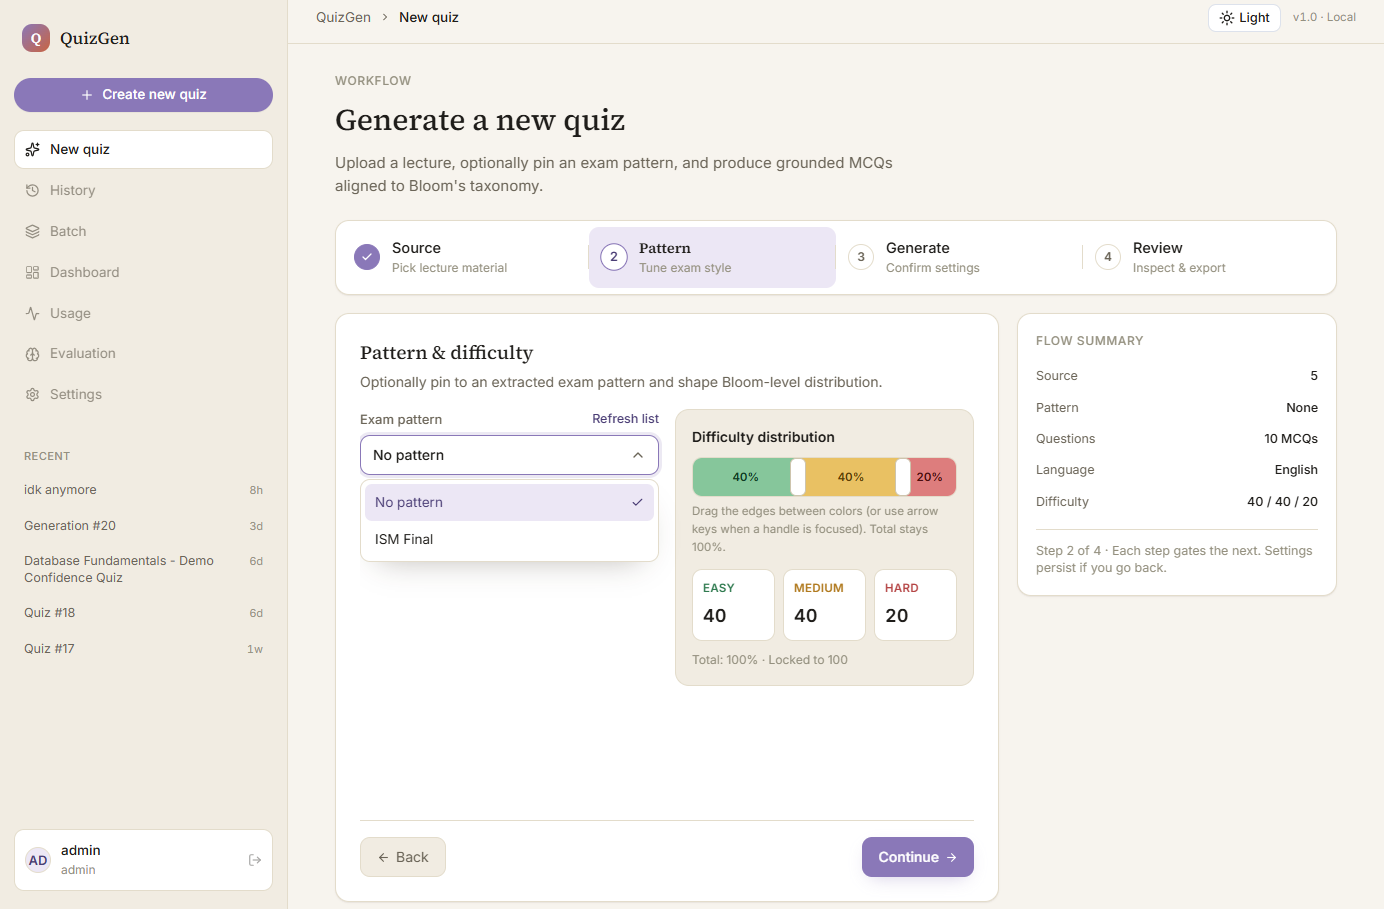
\includegraphics[width=0.92\linewidth]{02-workflow-pattern.png}
  \caption{Exam pattern and difficulty configuration step in the QuizGen wizard.}
  \label{fig:pattern-step}
\end{figure}

\subsection{MCQ Generation Method}

The generation prompt is built from four parts. The first part is the
retrieved source chunks. The second part is the generation request, such as
question count, question type, and language. The third part is the
difficulty distribution. The fourth part is the optional exam-pattern block
with sample questions and style information.

The assembled prompt is sent through the LLM router. The primary provider
is Groq with \textit{llama-3.3-70b-versatile}. The prompt asks for a JSON
array only, because the frontend and database cannot use a free-form essay
response. In practice, this strict schema is necessary: during development,
LLM responses sometimes included markdown fences, extra explanation text, or
missing fields. The parser therefore has to validate and normalize the
response before storing it.

The fourth part, pattern examples, was added specifically because early
generation runs produced questions that were technically grounded but did not
match the style I expected. Without sample questions in the prompt, the model
defaulted to short definition questions even when the topic called for
application or scenario questions. Placing sample exam questions under the
heading \textit{Example Questions} gave the model a concrete style reference
that the difficulty distribution label alone could not provide.

The backend stores the actual prompt template in the following source file:
\path{backend/app/prompts/v1/question_generation.py}. A shortened excerpt is
shown below, preserving the implemented placeholders:

\begin{verbatim}
## Source Material
{retrieved_chunks_joined_with_separators}

## Generation Instructions
- Generate exactly {num_questions} questions
- Question types to include: {question_types}
- Language: {language}
- Prompt version: v1

## Difficulty Distribution (MUST follow exactly)
- {level}: {percentage}% (~{count} questions)

## Pattern Requirements
- Question type distribution: {pattern_config.question_types}
- Average question length: ~{pattern_config.avg_length} words

## Example Questions (match this style and format):
Example 1:
{sample_question}

## Output Format
Return a JSON array of objects with question, options, answer,
explanation, difficulty, and bloom_level.
\end{verbatim}

The generation provider is called through \texttt{llm\_router.py}. Gemini
and Groq requests use temperature 0.7. I used this setting to allow some
variation in stems and distractors while still relying on source material,
schema constraints, and difficulty instructions. The application generation
path does not set a fixed random seed, so each generation stores prompt
version, provider, token usage, and configuration snapshot for later
inspection.

\begin{table}[H]
  \centering
  \singlespacing
  \caption{MCQ output schema.}
  \label{tab:mcq-schema}
  \begin{tabular}{@{}p{3.7cm}p{2.2cm}p{7.1cm}@{}}
    \toprule
    \textbf{Field} & \textbf{Type} & \textbf{Description} \\
    \midrule
    \texttt{type}        & string  & Question type: \texttt{mcq}, \texttt{true\_false}, \texttt{fill\_blank} \\
    \texttt{question}    & string  & The question stem \\
    \texttt{options}     & array   & Four labelled options (A–D) for MCQ; empty otherwise \\
    \texttt{answer}      & string  & The correct answer \\
    \texttt{explanation} & string  & Brief explanation referencing the source material \\
    \texttt{difficulty}  & string  & \texttt{easy}, \texttt{medium}, or \texttt{hard} \\
    \texttt{bloom\_level} & string & One of six Bloom levels (see Section~\ref{subsec:bloom}) \\
    \bottomrule
  \end{tabular}
\end{table}

The Bloom level field is generated by the LLM and then checked by the
backend against the allowed labels. The valid values are
\texttt{remember}, \texttt{understand}, \texttt{apply}, \texttt{analyze},
\texttt{evaluate}, and \texttt{create}. The system asks the model to follow
the requested difficulty distribution, but the evaluation in Chapter~V shows
that this control is not perfect.

\subsection{Prompt Assembly and Output Validation}

The prompt assembly stage converts user choices and retrieved chunks into
one instruction. I keep the order stable: role, source material, optional
pattern examples, constraints, output schema, and validation rules. The
order is deliberate. Small prompt changes produce different questions, so
the prompt version is part of the reproducibility record.

The parser is also part of the design, not just an error handler. After the
model returns a response, the \texttt{question\_generator} service removes
common markdown wrappers, tries to parse JSON, extracts a JSON array if the
provider adds extra text, and repairs common issues such as trailing commas.
If this still fails, the system asks the provider for a JSON-only repair
response. If the retry also fails, the generation is marked as failed and
the frontend shows the error.

The parser prioritizes usability over strictness. It assigns an id, forces
the type to \texttt{mcq}, truncates options to four entries, keeps answer
and explanation fields when present, defaults missing difficulty to
\texttt{medium}, and maps invalid Bloom labels from difficulty. This is a practical compromise. Strict rejection would make the demo fail on malformed responses;
lenient normalization keeps usable questions while leaving final review
to the lecturer.

Table~\ref{tab:prompt-validation} summarizes the major parsing and
normalization behaviours applied before a generated question is stored.

\begin{table}[H]
  \centering
  \singlespacing
  \caption{Prompt output parsing and normalization behaviour.}
  \label{tab:prompt-validation}
  \small
  \begin{tabular}{@{}p{5.2cm}p{8.2cm}@{}}
    \toprule
    \textbf{Parser behaviour} & \textbf{Purpose} \\
    \midrule
    Response must parse as JSON & Prevents storing free-text LLM responses \\
    Dict/list wrappers are normalized & Handles common provider response shapes \\
    Non-dictionary items are skipped & Prevents unusable primitive values from being stored \\
    Options are truncated to four entries & Matches the MCQ interface expectation \\
    Missing difficulty defaults to medium & Supports downstream grouping \\
    Invalid Bloom labels are remapped & Keeps Bloom labels inside allowed values \\
    Answer text is preserved for quiz scoring & Allows later answer canonicalization \\
    \bottomrule
  \end{tabular}
\end{table}

The backend validates JSON format and field presence, but final
pedagogical quality still depends on the generated content and lecturer
review. Automation handles structure; human review handles pedagogy.

\subsection{Grounding and Hallucination Proxy}
\label{subsec:grounding}

After generation, each MCQ can be scored by the grounding evaluator. This
score is only a proxy. It estimates whether the question, answer, and
explanation are semantically close to the source material. It does not prove
that the answer key is correct. I still include it because it gives the
lecturer a fast way to find questions that need more checking.

The evaluator concatenates the question text, correct answer, and
explanation, embeds this passage, and compares it with the source document
embedding. Because raw cosine similarity lies in $[-1, 1]$, it is normalized
to $[0, 1]$ using $s = (\text{cos} + 1) / 2$ before applying thresholds.

More formally, for a generated question $q_i$, the evaluator builds:
\[
  p_i = \text{question}_i \; || \; \text{answer}_i \; || \; \text{explanation}_i
\]
where $||$ denotes string concatenation. It then embeds $p_i$ and the source
document text into vectors $\mathbf{p}_i$ and $\mathbf{d}$. The raw semantic
score is:
\[
  \cos(\mathbf{p}_i, \mathbf{d}) =
  \frac{\mathbf{p}_i \cdot \mathbf{d}}
       {\|\mathbf{p}_i\| \|\mathbf{d}\| + 10^{-12}}
\]
and the reported grounding score is:
\[
  s_i = \max(0, \min(1, (\cos(\mathbf{p}_i, \mathbf{d}) + 1) / 2)).
\]
For example, if a generated DBMS question and its explanation produce a raw
cosine similarity of 0.46 against the uploaded database lecture text, the
normalized grounding score is $(0.46 + 1) / 2 = 0.73$, which falls into the
\texttt{well\_grounded} range. If a different question produces a raw cosine
similarity of -0.10, the normalized score is 0.45 and the item is flagged as
\texttt{poorly\_grounded}. These values should be read as review hints only.
They help the reviewer notice weak source support, but they do not certify
the factual correctness of the answer.

Table~\ref{tab:grounding} lists the three grounding status levels and their
corresponding score ranges.

\begin{table}[H]
  \centering
  \singlespacing
  \caption{Grounding status levels and semantic score thresholds.}
  \label{tab:grounding}
  \small
  \begin{tabular}{@{}p{3.4cm}p{2.6cm}p{7.4cm}@{}}
    \toprule
    \textbf{Status} & \textbf{Score range} & \textbf{Interpretation} \\
    \midrule
    \texttt{well\_grounded}      & $s > 0.70$          & Strong semantic overlap with source \\
    \texttt{partially\_grounded} & $0.45 < s \leq 0.70$ & Moderate overlap; review recommended \\
    \texttt{poorly\_grounded}    & $s \leq 0.45$        & Weak overlap; likely unsupported \\
    \bottomrule
  \end{tabular}
\end{table}

The evaluator also computes keyword overlap — a cruder signal than
embedding similarity but easier to inspect at a glance. Together, the
semantic score and keyword overlap help identify suspicious questions.
They are review aids, not automatic proof of correctness.

\subsection{Quiz Practice and Confidence Trend}

After review, a generation becomes a named quiz. The practice page shows one
question at a time, stores the selected answer, and tracks elapsed time. On
submission, the backend writes the attempt to \texttt{quiz\_attempts} with
the generation id, answers, score, time, and Bloom-level correctness. Each
question also carries a short topic label, so later dashboard pages can
summarize practice performance by topic and not only by Bloom level.

For this thesis, the confidence trend is kept simple: a chronological
sequence of attempt score percentages for the user. It does not yet group
the series by quiz, which is a dashboard limitation I document rather than
present as a finished feature. Even so, it gives a quick read on whether
practice scores are improving or declining over time.

The topic review feature uses the same stored attempts. The backend endpoint
\texttt{/api/dashboard/topic-stats} reads the saved answers, compares them
with the correct answers, groups the result by question topic, and marks a
topic as weak when its accuracy is below 70\%. If the generation was created
from a focused topic practice request, the backend keeps that focus label in
the stored configuration and applies it to the questions during aggregation.
This avoids splitting one focused practice quiz into many small topic names.
From the dashboard, a weak topic can create a new practice quiz from the
same source document by sending \texttt{topic\_focus} to the generation
endpoint.

Figure~\ref{fig:practice-sequence} shows the practice and confidence trend
workflow.

\begin{figure}[H]
  \centering
  \singlespacing
  \fbox{%
    \begin{minipage}{0.82\linewidth}
      \centering
      \vspace{0.3cm}
      User selects a named quiz from history\\[4pt]
      $\downarrow$\\[4pt]
      Frontend loads questions from generation record\\[4pt]
      $\downarrow$\\[4pt]
      User answers each question; timer runs\\[4pt]
      $\downarrow$\\[4pt]
      POST \texttt{/api/quiz/submit} $\rightarrow$ score stored in \texttt{quiz\_attempts}\\[4pt]
      $\downarrow$\\[4pt]
      User opens Dashboard\\[4pt]
      $\downarrow$\\[4pt]
      GET \texttt{/api/dashboard/trend} $\rightarrow$ chronological attempts for user\\[4pt]
      $\downarrow$\\[4pt]
      GET \texttt{/api/dashboard/topic-stats} $\rightarrow$ topic mastery and weak topics\\[4pt]
      $\downarrow$\\[4pt]
      Line chart, Bloom breakdown, and topic practice recommendation\\[0.3cm]
    \end{minipage}%
  }
  \caption{Quiz practice and confidence trend sequence.}
  \label{fig:practice-sequence}
\end{figure}

\subsection{Database Design}
\label{subsec:database-design}

The prototype stores all persistent data in one SQLite database.
SQLite is sufficient at thesis scale: one user at a time, a small document
set, and no concurrent write pressure.
Table~\ref{tab:entities} lists each entity and its purpose.

\begin{table}[H]
  \centering
  \singlespacing
  \caption{Database entities and their roles.}
  \label{tab:entities}
  \small
  \begin{tabular}{@{}p{3.9cm}p{9.5cm}@{}}
    \toprule
    \textbf{Entity} & \textbf{Role} \\
    \midrule
    \texttt{users}            & Account identity, hashed password, and role \\
    \texttt{documents}        & Uploaded files, raw text, and processed chunks \\
    \texttt{chunk\_embeddings} & Chunk vectors for semantic retrieval \\
    \texttt{patterns}         & Exam templates, sample questions, style config \\
    \texttt{generations}      & Generated quiz records with prompt and config snapshot \\
    \texttt{quiz\_attempts}   & User answers, scores, timing, and Bloom accuracy \\
    \texttt{batch\_jobs}      & Batch generation status, progress, and per-document results \\
    \texttt{api\_calls}       & Provider usage, token count, and latency logs \\
    \bottomrule
  \end{tabular}
\end{table}

The key relationships are as follows. A \texttt{user} owns many
\texttt{documents} and \texttt{patterns}. A \texttt{generation} references
one \texttt{document} (as source) and optionally one \texttt{pattern} (as
style guide). A \texttt{quiz\_attempt} references one \texttt{generation}
and one \texttt{user}. A \texttt{batch\_job} references a user and stores
the list of document identifiers processed as independent generations. The
\texttt{api\_calls} table records every outbound LLM and embedding call for
usage tracking and provider-level diagnostics.

\begin{figure}[H]
  \centering
  \singlespacing
  \fbox{%
    \begin{minipage}{0.88\linewidth}
      \centering
      \vspace{0.3cm}
      \small
      \begin{tabular}{ccccc}
        \texttt{USERS} & $\longrightarrow$ & \texttt{DOCUMENTS} & $\rightarrow$ & \texttt{CHUNK\_EMBEDDINGS} \\[4pt]
        $\downarrow$ & & $\downarrow$ & & \\[4pt]
        \texttt{PATTERNS} & $\rightarrow$ & \texttt{GENERATIONS} & $\rightarrow$ & \texttt{QUIZ\_ATTEMPTS} \\[4pt]
        & & $\uparrow$ & & \\[4pt]
        & & \texttt{API\_CALLS} & & \\[4pt]
      \end{tabular}
      \vspace{0.2cm}
      \par\small Arrow ($\rightarrow$) denotes a foreign-key reference from child to parent.
      \vspace{0.2cm}
    \end{minipage}%
  }
  \caption{Simplified entity--relationship overview of the QuizGen database.}
  \label{fig:er-diagram}
\end{figure}

The \texttt{generations} table stores a \texttt{config\_snapshot} JSON
field. It records the chunk size, embedding model, prompt version, and
provider used for the run. This was added so that evaluation outputs in
Chapter~V can be traced back to the system configuration that produced
them.

\subsection{Security and Reproducibility Considerations}

Even a thesis prototype handles real data: uploaded lecture files,
generated questions, and student attempts. So I added basic security
controls. Passwords are hashed, API calls use JWT bearer
tokens, and protected routes resolve the current user on the backend. The
frontend cannot choose another user's id and read their data through normal
API calls.

I validate uploads by extension and size before processing.
Unsupported formats are rejected. API keys and JWT secrets are loaded from
environment variables instead of being hard-coded. These controls are not a
complete production security design, but they are enough for the local
prototype used in this thesis.

Reproducibility is handled by saved configuration and result artifacts. Each
generation stores prompt version, provider, model, source document, optional
pattern, selected difficulty settings, and generated payload. The evaluation
runner stores CSV outputs, aggregate comparison tables, failure-analysis
reports, and checkpoint JSONL records. These files helped me recover and
inspect long runs when quota or timeout issues interrupted the process.

The main limitation is that external LLM APIs can change over time. Even
with the same prompt and evaluation seed, provider-side updates may produce
different outputs. The thesis therefore reports the cached evaluation run
used for the final comparison. OpenRouter auto-free and local Ollama
fallback improve demonstration resilience, but they are engineering support,
not the main research contribution.

\clearpage
\section{Implementation and Results}

\subsection{Development Environment}

In this implementation, QuizGen is a two-tier web application. The backend
is written in Python with FastAPI, and the frontend is written with Next.js
and React. I kept the two parts separate because the backend has to manage
documents, embeddings, LLM calls, and storage, while the frontend has to
guide the user through upload, pattern setup, generation, review, and
practice. Table~\ref{tab:tech-stack} lists the technology stack used in the
implementation.

\begin{table}[H]
  \centering
  \singlespacing
  \caption{QuizGen technology stack.}
  \label{tab:tech-stack}
  \small
  \begin{tabular}{@{}p{3.0cm}p{3.4cm}p{7.0cm}@{}}
    \toprule
    \textbf{Layer} & \textbf{Technology} & \textbf{Notes} \\
    \midrule
    Backend language    & Python 3.10+             & \\
    Backend framework   & FastAPI                  & RESTful API, JWT authentication \\
    ASGI server         & Uvicorn                  & Hot-reload in development \\
    Database            & SQLite                   & Single-file, zero-configuration \\
    Frontend framework  & Next.js + React          & App Router, TypeScript \\
    UI components       & shadcn/ui + Tailwind CSS & \\
    Charts              & Recharts + custom SVG    & Evaluation trends, confidence trend, Bloom breakdown \\
    LLM primary         & Groq API                 & \textit{llama-3.3-70b-versatile} \\
    LLM fallbacks       & Groq API (multiple)      & Four alternative Groq models \\
    LLM cloud fallback  & Gemini + OpenRouter      & Gemini legacy path and OpenRouter auto-free models \\
    LLM local fallback  & Ollama                   & \textit{gemma4:e4b-it-q4\_K\_M}, offline \\
    Embeddings          & Gemini + OpenRouter      & \textit{gemini-embedding-001}; OpenRouter fallback model \\
    Local run           & \texttt{start-all.bat}   & Starts both services on Windows \\
    Containerization    & Docker Compose           & Two-service stack with named volume \\
    \bottomrule
  \end{tabular}
\end{table}

For local development on Windows, I used \texttt{start-all.bat} to start
both services. The backend runs on port 8000 and the frontend runs on port
3000. Docker Compose is also included for a two-service setup with a named
SQLite volume. FastAPI exposes Swagger documentation at
\texttt{http://localhost:8000/docs}, which was useful while checking API
requests during implementation.

\subsection{Project Structure and Configuration}

The repository is split into backend, frontend, evaluation, and
documentation directories. Keeping web app code under backend and frontend, and evaluation
scripts under eval, prevented thesis evidence from mixing with product
code. For example, the web app lives under backend and
frontend, while evaluation outputs and thesis notes stay under
\texttt{eval} and \texttt{doc/thesis}. Table~\ref{tab:project-structure}
summarizes the major directories and their roles.

\begin{table}[H]
  \centering
  \singlespacing
  \caption{Repository structure used by the QuizGen implementation.}
  \label{tab:project-structure}
  \small
  \begin{tabular}{@{}p{4.8cm}p{8.6cm}@{}}
    \toprule
    \textbf{Path} & \textbf{Responsibility} \\
    \midrule
    \texttt{backend/app/api} & FastAPI route modules for user-facing endpoints \\
    \texttt{backend/app/services} & Document processing, retrieval, generation, evaluation logic \\
    \texttt{backend/app/models} & Database model definitions and persistence objects \\
    \texttt{backend/app/schemas} & Request and response schemas used by the API layer \\
    \texttt{frontend/src/app} & Next.js pages and route-level application layout \\
    \texttt{frontend/src/components} & Reusable workflow and UI components \\
    \texttt{frontend/src/features} & Feature-specific views such as dashboard and evaluation \\
    \texttt{eval} & Reproducible evaluation runner, dataset, and result outputs \\
    \texttt{doc/thesis} & Thesis manuscript, evaluation notes, and documentation artifacts \\
    \bottomrule
  \end{tabular}
\end{table}

Configuration is mainly controlled through environment variables, including
\texttt{DATABASE\_PATH}, \texttt{JWT\_SECRET}, provider API keys, upload
size, and the fallback chain. This allowed me to run UI smoke tests with
dummy keys and real generation tests with actual keys. The frontend keeps
API access in \texttt{frontend/src/lib/api.ts}, where bearer tokens and
error handling are centralized.

\subsection{Backend Implementation}

The backend is organised into two main layers. API routers handle HTTP
requests, while service modules contain the main business logic. This keeps
the route code shorter and makes each technical step easier to explain in
the thesis. Table~\ref{tab:backend-modules} lists all modules and their
responsibilities.

\begin{table}[H]
  \centering
  \singlespacing
  \caption{Backend API modules and services.}
  \label{tab:backend-modules}
  \small
  \begin{tabular}{p{1.4cm}p{4.2cm}p{7.8cm}}
    \toprule
    \textbf{Type} & \textbf{Module} & \textbf{Responsibility} \\
    \midrule
    Router & \texttt{auth}                  & Registration, login, JWT token issuance \\
    Router & \texttt{documents}             & Upload, text extraction, chunk storage \\
    Router & \texttt{patterns}              & Create, list, and delete exam patterns \\
    Router & \texttt{generations}           & Trigger MCQ generation, retrieve results \\
    Router & \texttt{batch}                 & Batch jobs that create independent quizzes per document \\
    Router & \texttt{quiz}                  & Submit attempts, retrieve attempt records \\
    Router & \texttt{dashboard}             & Confidence trend and Bloom breakdown data \\
    Router & \texttt{usage}                 & API call logs and provider status \\
    Router & \texttt{eval}                  & Serve latest and historical evaluation artifacts to admin dashboard \\
    Router & \texttt{settings}              & Return live model, fallback, and RAG configuration \\
    \midrule
    Service & \texttt{document\_processor}  & PDF/DOCX/PPTX extraction and chunking \\
    Service & \texttt{embedder}             & Batch embedding through the configured embedding router \\
    Service & \texttt{chunk\_selector}      & Cosine-similarity retrieval of top-$k$ chunks \\
    Service & \texttt{pattern\_analyzer}    & Parse and validate exam-pattern JSON \\
    Service & \texttt{question\_generator}  & Prompt assembly, LLM call, and JSON parsing \\
    Service & \texttt{question\_extractor}  & Extract sample questions from uploaded patterns \\
    Service & \texttt{accuracy\_evaluator}  & Grounding score computation \\
    Service & \texttt{llm\_router}          & Provider fallback chain and API call logging \\
    Service & \texttt{batch\_processor}     & Placeholder for future extraction of batch orchestration logic \\
    Service & \texttt{rate\_limit}          & Per-user request rate limiting \\
    \bottomrule
  \end{tabular}
\end{table}

The \texttt{main.py} entry point registers ten routers under the
\texttt{/api} prefix, enables CORS for the frontend, and initializes the
SQLite schema on startup. Protected endpoints use FastAPI dependencies to
resolve the current user from the JWT token.

The \texttt{llm\_router} service handles provider fallback. The default
chain starts with Groq \textit{llama-3.3-70b-versatile}, then tries other
Groq models, OpenRouter auto-free models, and finally local Ollama as the
last route. This was added because API quota and provider availability were
real issues during testing. Every outbound LLM and embedding call is logged
to \texttt{api\_calls}, so the usage dashboard can show provider, model,
latency, tokens, and status.

\subsection{API Workflow Implementation}

The API workflow follows the same order as the user interface. A user logs
in, uploads or selects a document, optionally selects a pattern, and then
submits a generation request. After generation, the quiz can be opened from
history or attempted through the quiz route. I kept this order the same in
the API and frontend because it made debugging the wizard easier.

Table~\ref{tab:api-workflow} lists representative endpoints used in the
main workflow.

\begin{table}[H]
  \centering
  \singlespacing
  \caption{Representative API endpoints in the QuizGen workflow.}
  \label{tab:api-workflow}
  \small
  \begin{tabular}{@{}p{4.4cm}p{1.6cm}p{7.4cm}@{}}
    \toprule
    \textbf{Endpoint} & \textbf{Method} & \textbf{Purpose} \\
    \midrule
    \texttt{/api/auth/register} & POST & Create a new user account \\
    \texttt{/api/auth/login} & POST & Return a JWT access token \\
    \texttt{/api/documents/upload} & POST & Upload and process lecture material \\
    \texttt{/api/documents/} & GET & List documents owned by the current user \\
    \texttt{/api/patterns/} & POST & Create an exam-pattern record \\
    \texttt{/api/generations/} & POST & Generate a question set from source material \\
    \texttt{/api/generations/} & GET & List previous generations and titles \\
    \texttt{/api/quiz/submit} & POST & Submit answers for a generated quiz \\
    \texttt{/api/dashboard/trend} & GET & Return confidence trend data \\
    \texttt{/api/usage/} & GET & Return provider usage statistics \\
    \bottomrule
  \end{tabular}
\end{table}

The generation endpoint is the most complex route. It checks document
ownership, loads the selected pattern, builds the retrieval query, selects
chunks, builds the prompt, calls the LLM router, parses the JSON response,
computes review signals, and stores the generation. These steps are kept in
service modules so that retrieval, prompt assembly, and parsing can change
without rewriting the HTTP route.

The API also returns explicit error codes for common cases. Missing
documents or patterns return \texttt{404}, invalid titles return
\texttt{400}, missing tokens return \texttt{401}, and non-admin users cannot
read evaluation artifacts. These checks are simple, but they make the
frontend errors easier to understand during demo.

\subsection{Frontend Implementation}

I built the frontend with Next.js App Router and TypeScript. The interface
uses a route-based Atelier layout because the earlier tabbed workflow became
harder to manage when I added history, quiz practice, dashboard, usage
tracking, evaluation, settings, and batch generation. The shared
\texttt{AtelierShell} keeps the sidebar, breadcrumb, theme control, and
recent-generation list in one place. This helped me keep the main workflow
cleaner while still letting users move back to old generations.

The main creation flow stays as a four-step wizard: Source, Pattern,
Generate, and Review. I kept this order because generation should not happen
before the source document and optional exam pattern are clear. The Source
step lets the user upload a lecture file or select a previously processed
document, as shown in Figure~\ref{fig:source-step}. This step was important
during testing because long filenames and repeated uploaded documents could
easily make the interface messy if the document selection page was not clear.

\begin{figure}[H]
  \centering
  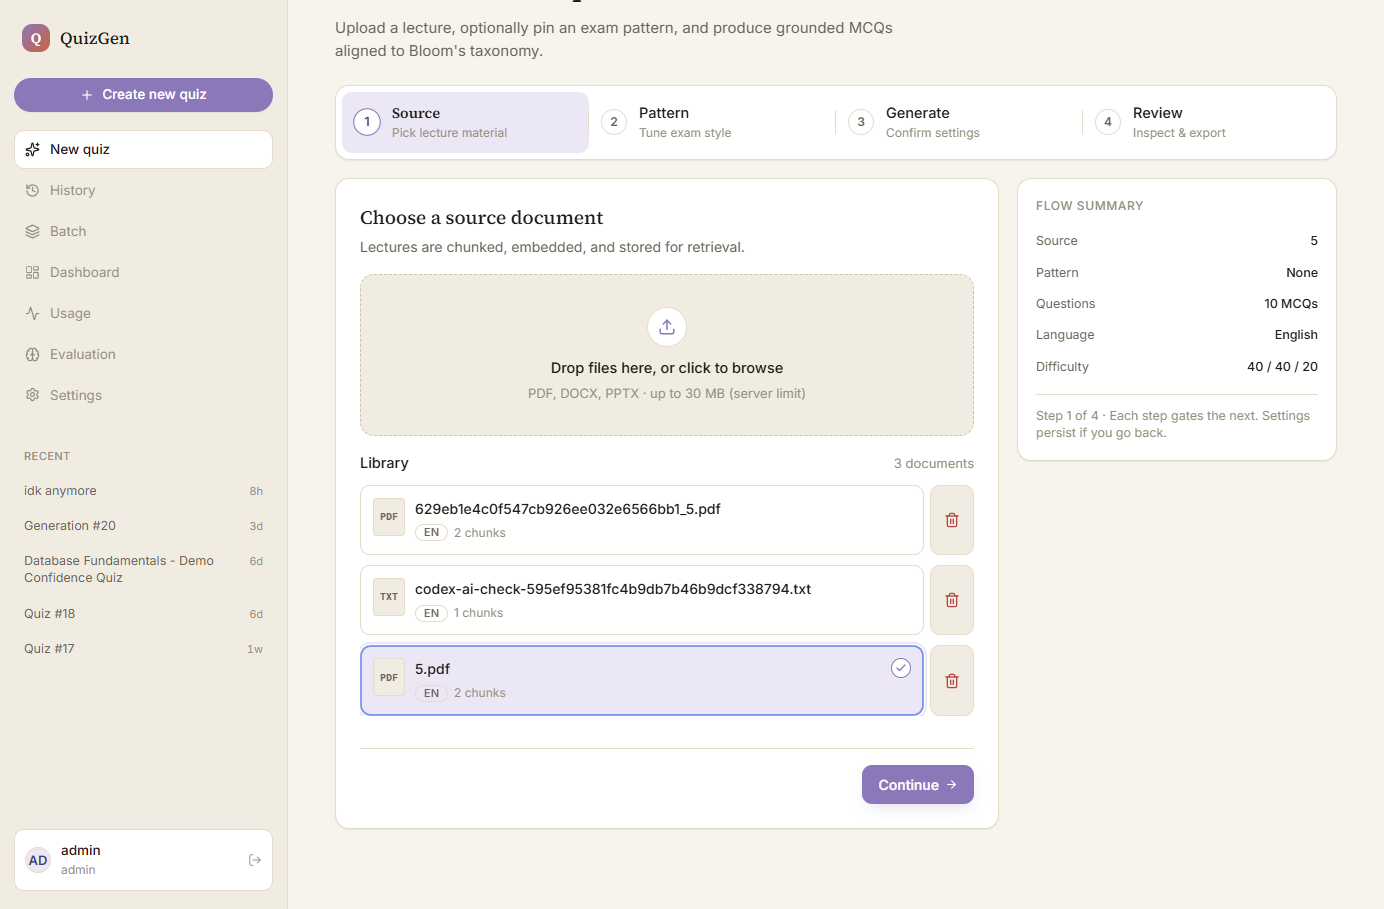
\includegraphics[width=0.95\linewidth]{01-workflow-source.png}
  \caption{Source step: document upload and selection in the QuizGen wizard.}
  \label{fig:source-step}
\end{figure}

The Pattern step connects the frontend to the few-shot part of the system.
If the user selects an exam pattern, the generation request includes the
saved sample-question style and difficulty configuration. If the user leaves
the pattern empty, the system still works, but the prompt only uses
retrieved lecture chunks and normal difficulty settings. I used this
fallback to make the app usable even when a lecturer has no old exam pattern
available.

The Generate step, shown in Figure~\ref{fig:generate-step}, asks the user
to confirm the selected source, optional pattern, question count, language,
and difficulty distribution before calling the backend. I kept this
confirmation screen because the generation call uses external LLM APIs and
can consume quota. The user should see the final setup before sending the
request.

\begin{figure}[H]
  \centering
  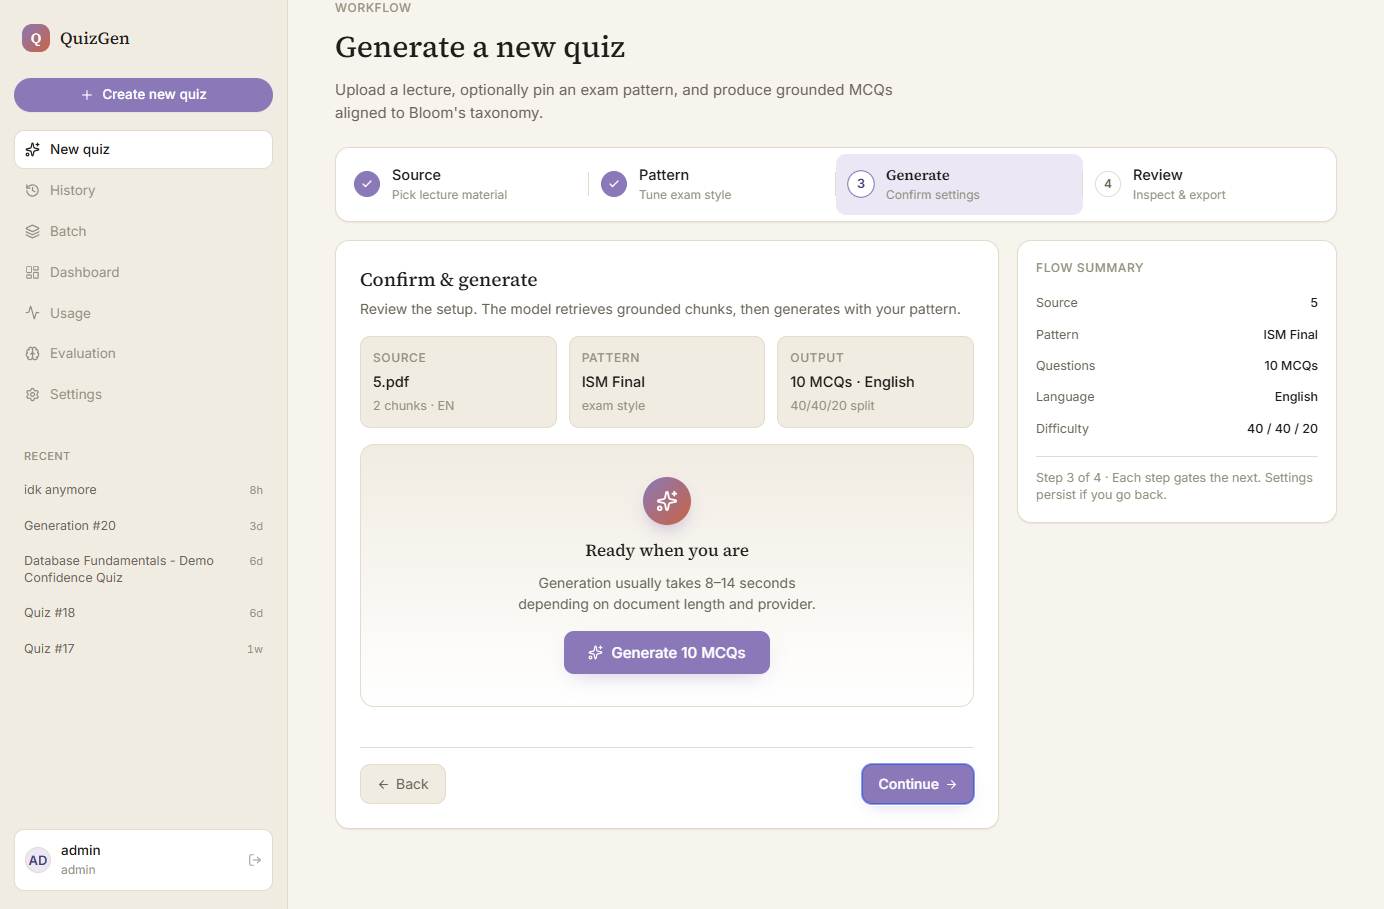
\includegraphics[width=0.95\linewidth]{03-workflow-generate-title.png}
  \caption{Generate step: quiz title assignment before submitting the
           generation request.}
  \label{fig:generate-step}
\end{figure}

The Review step is where the generated content becomes useful to a lecturer
or student. Figure~\ref{fig:review-step} shows the generated questions with
answer options, difficulty labels, Bloom labels, and grounding status. From
this page, the user can rename the saved generation, export it, run the
optional LLM grounding check again, or open it as a practice quiz. This page
is also the main reason why I did not treat generation as the final step.
The generated MCQs still need review before students use them.

\begin{figure}[H]
  \centering
  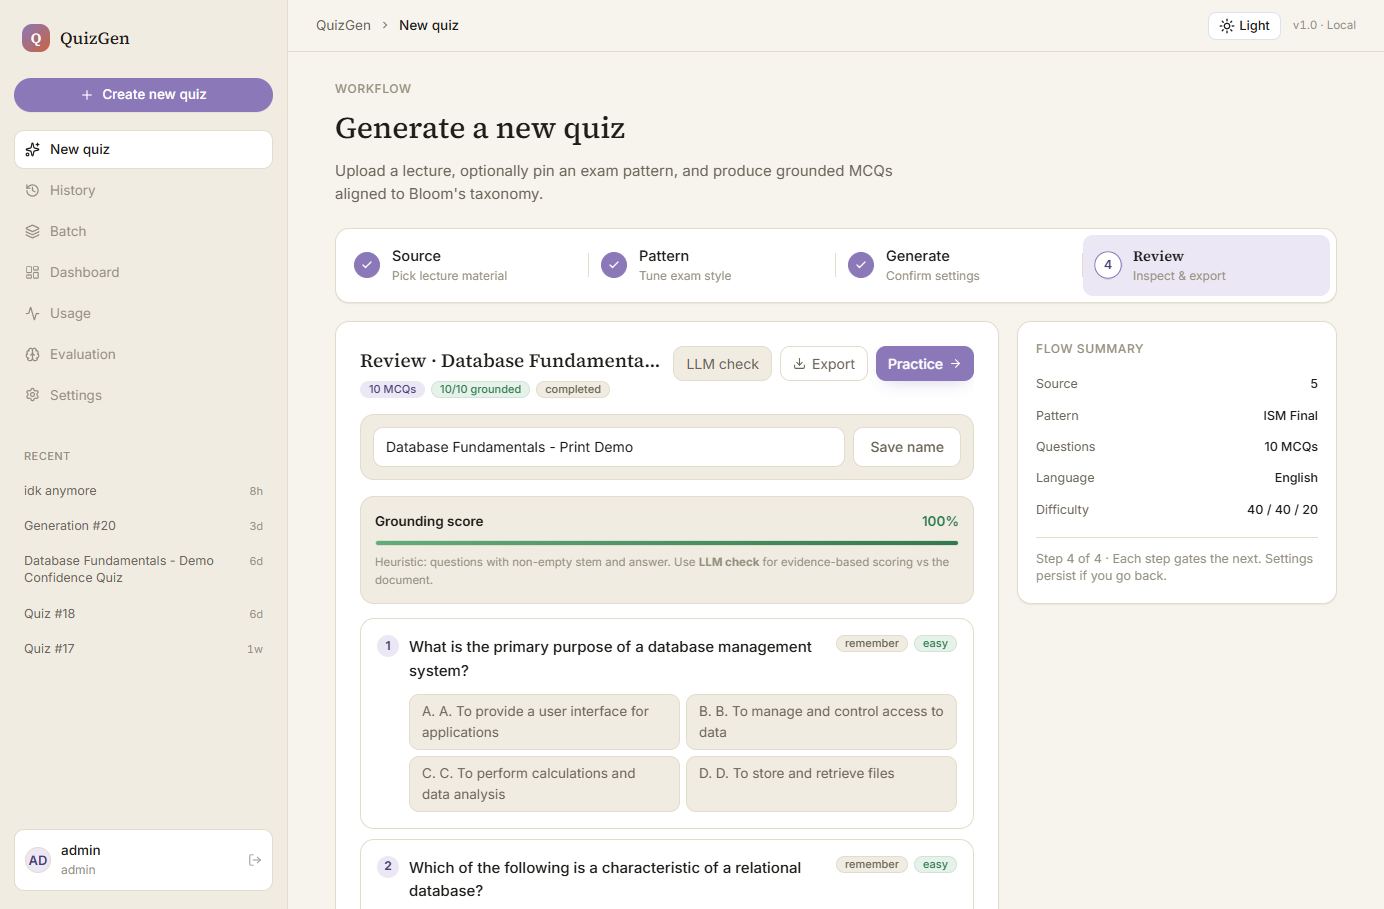
\includegraphics[width=0.95\linewidth]{04-workflow-review.png}
  \caption{Review step: generated quiz with grounding status, Bloom labels,
           and difficulty indicators.}
  \label{fig:review-step}
\end{figure}

The frontend keeps state across the wizard because each step depends on the
earlier step. The Source step stores the selected document. The Pattern step
stores either a selected pattern or an explicit no-pattern choice. The
Generate step stores count, language, and difficulty distribution. The Review
step stores the generated payload, editable title, export state, and
grounding results. I added guards to stop invalid requests before they reach
the backend. A user cannot continue without a source document, the
difficulty percentages are checked before generation, and the question count
is bounded.

I also added visible error handling because external providers failed during
testing. If upload fails, the user stays on the Source step. If generation
fails because of quota, JSON parsing, or validation, the Generate step shows
the error and allows a retry. This made the demo workflow less fragile
because the user did not have to restart the whole process after one failed
API call.

Navigation uses an \texttt{auth-provider} context. It stores the token and
attaches it to API requests. Users without a token are redirected to login.
Toast notifications show quota warnings and API errors without blocking the
interface.

\subsection{Quiz Practice Implementation}

After a generation is saved, it appears in history and in the recent
sidebar. The user can open it as a timed quiz through
\texttt{/quiz/[genId]}. This page loads the saved generation record, shows
one question at a time, stores the selected answer, and runs an elapsed-time
counter. I used this design to make the generated MCQs feel like a real
practice activity instead of a static text list.

\begin{figure}[H]
  \centering
  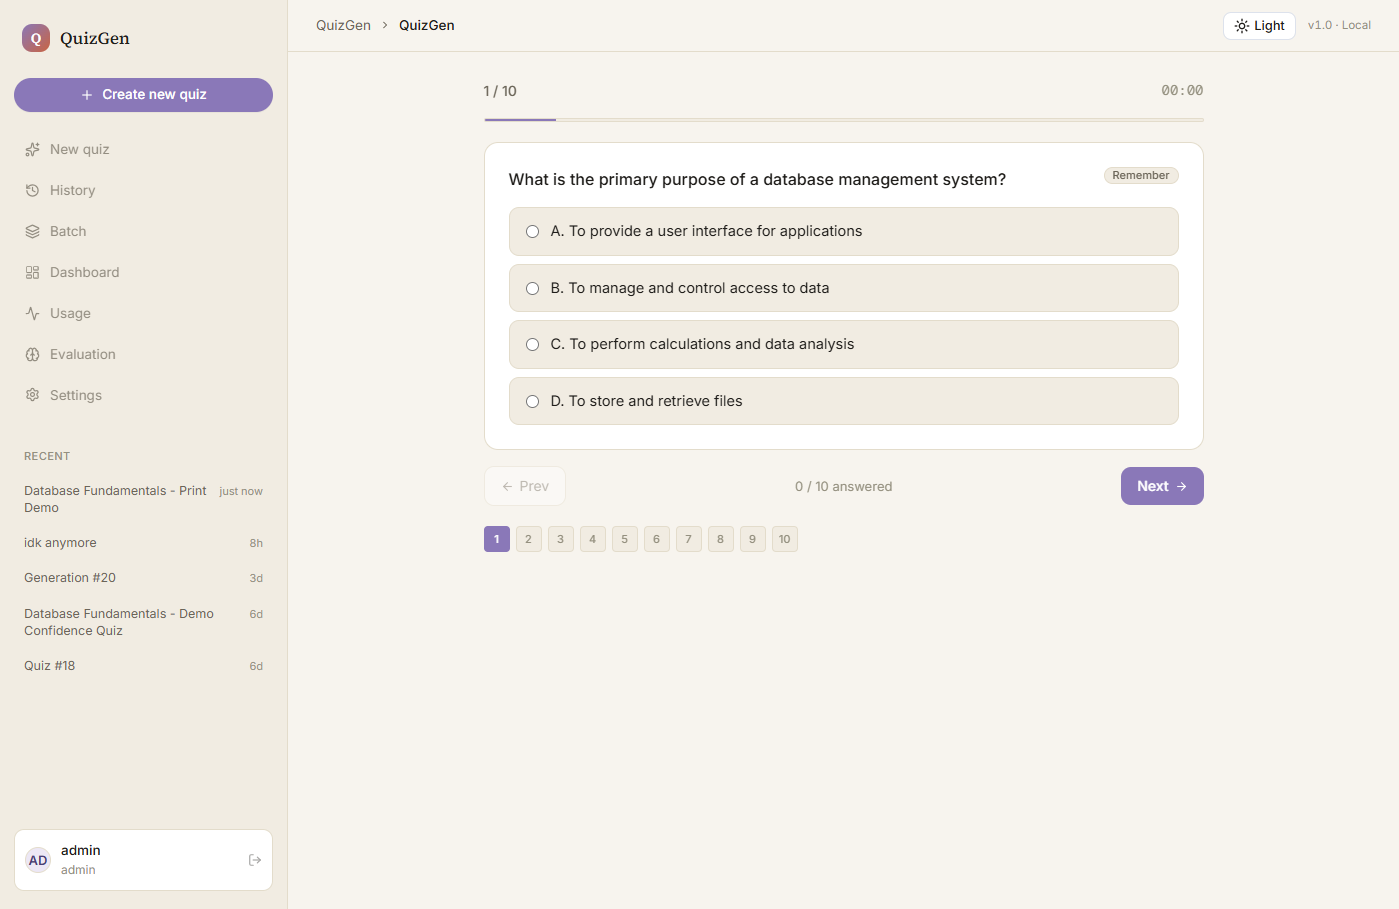
\includegraphics[width=0.95\linewidth]{05-quiz-practice.png}
  \caption{Quiz practice interface showing a question with answer options
           and the elapsed timer.}
  \label{fig:quiz-practice}
\end{figure}

When the user submits the quiz, the frontend calls
\texttt{POST /api/quiz/submit}. The backend stores the attempt in
\texttt{quiz\_attempts} with the generation id, selected answers, score,
elapsed time, and Bloom-level correctness. After submission, the user is
redirected to \texttt{/quiz/attempt/[attemptId]}. This page shows the
selected answer, correct answer, explanation, and Bloom level for each
question. This closes the loop from generation to actual self-practice.

\begin{figure}[H]
  \centering
  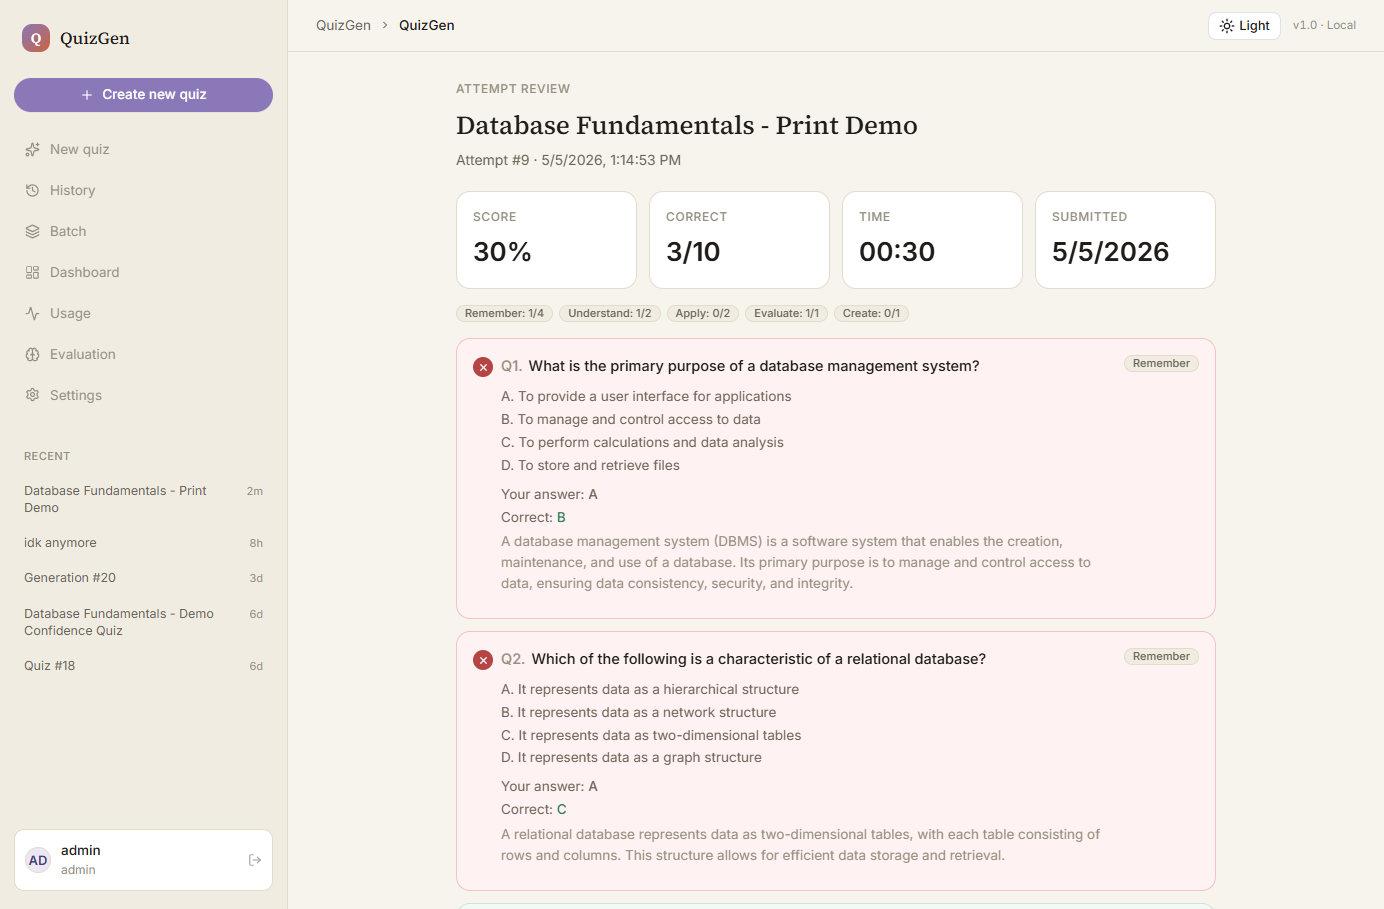
\includegraphics[width=0.95\linewidth]{06-attempt-review.png}
  \caption{Attempt review page showing per-question correctness, correct
           answers, explanations, and Bloom levels.}
  \label{fig:attempt-review}
\end{figure}

\subsection{Dashboard and Usage Implementation}

The dashboard reads saved attempts through the dashboard API and turns them
into practice feedback. I do not present this dashboard as production-grade
multi-user analytics. In this thesis version, it mainly shows a confidence
trend, recent attempts, Bloom breakdown, and topic mastery review. This
limitation is important because the dashboard still summarizes a small local
prototype, not a real classroom deployment.

Figure~\ref{fig:history-rename} shows the generation history panel. I
included the inline rename function because generated quizzes often need a
clearer title after review. During testing, default generation names were
hard to read in the sidebar, so renaming helped keep repeated test runs
usable.

\begin{figure}[H]
  \centering
  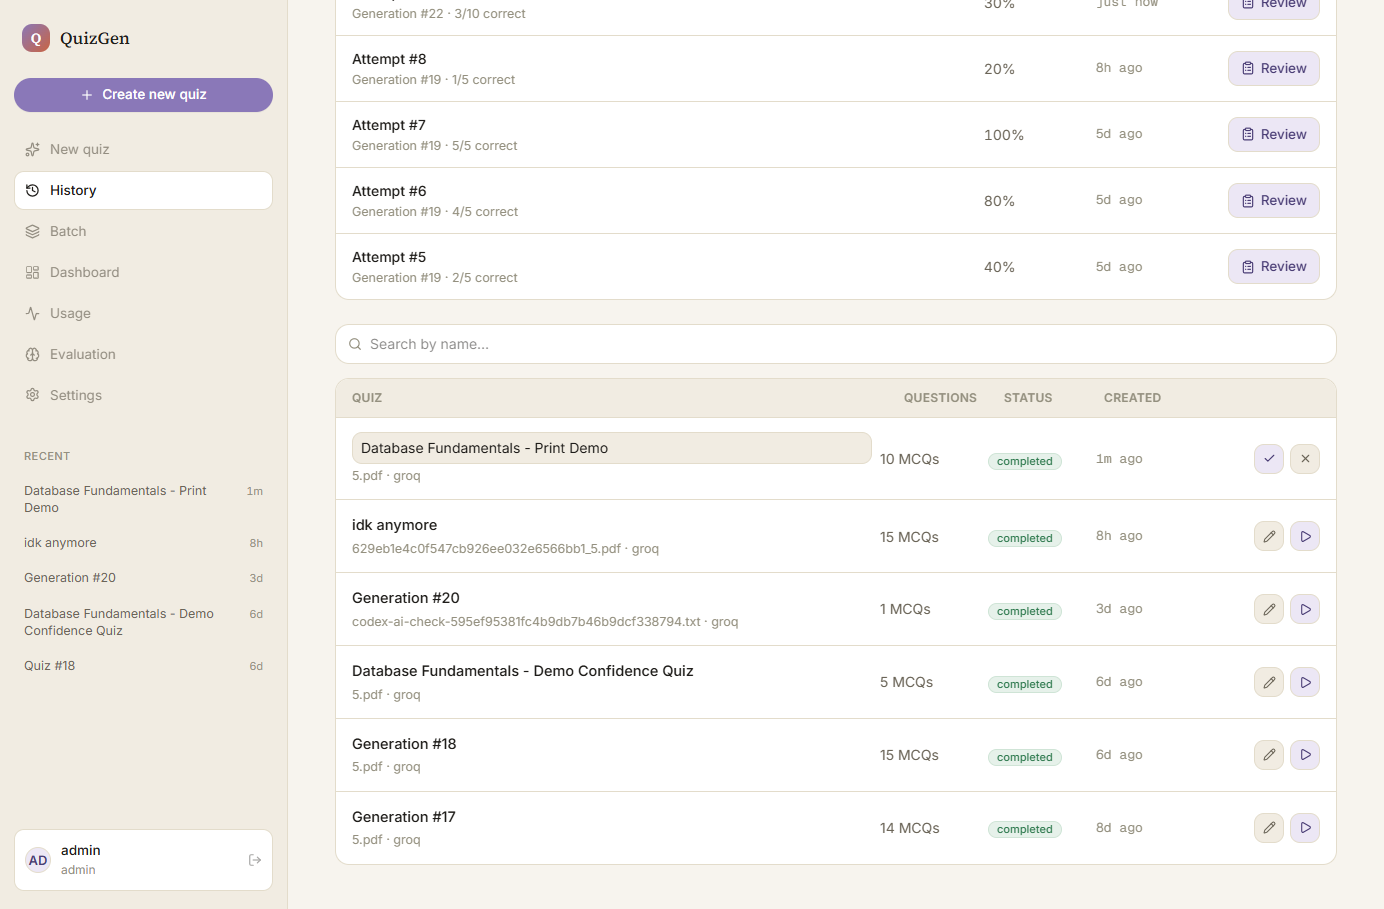
\includegraphics[width=0.95\linewidth]{07-history-rename.png}
  \caption{Generation history panel with inline quiz rename functionality.}
  \label{fig:history-rename}
\end{figure}

Figure~\ref{fig:confidence-trend} shows the dashboard view for confidence
trend and topic-based review. The topic mastery panel counts correct and
total answers for each topic, marks topics below 70\% accuracy as weak, and
enables a \textit{Practice topic} action. That action calls the normal
generation endpoint with the original document id, six MCQ questions, and
the selected \texttt{topic\_focus}. This is the part that turns a weak
dashboard result into a new focused quiz from the same document.

\begin{figure}[H]
  \centering
  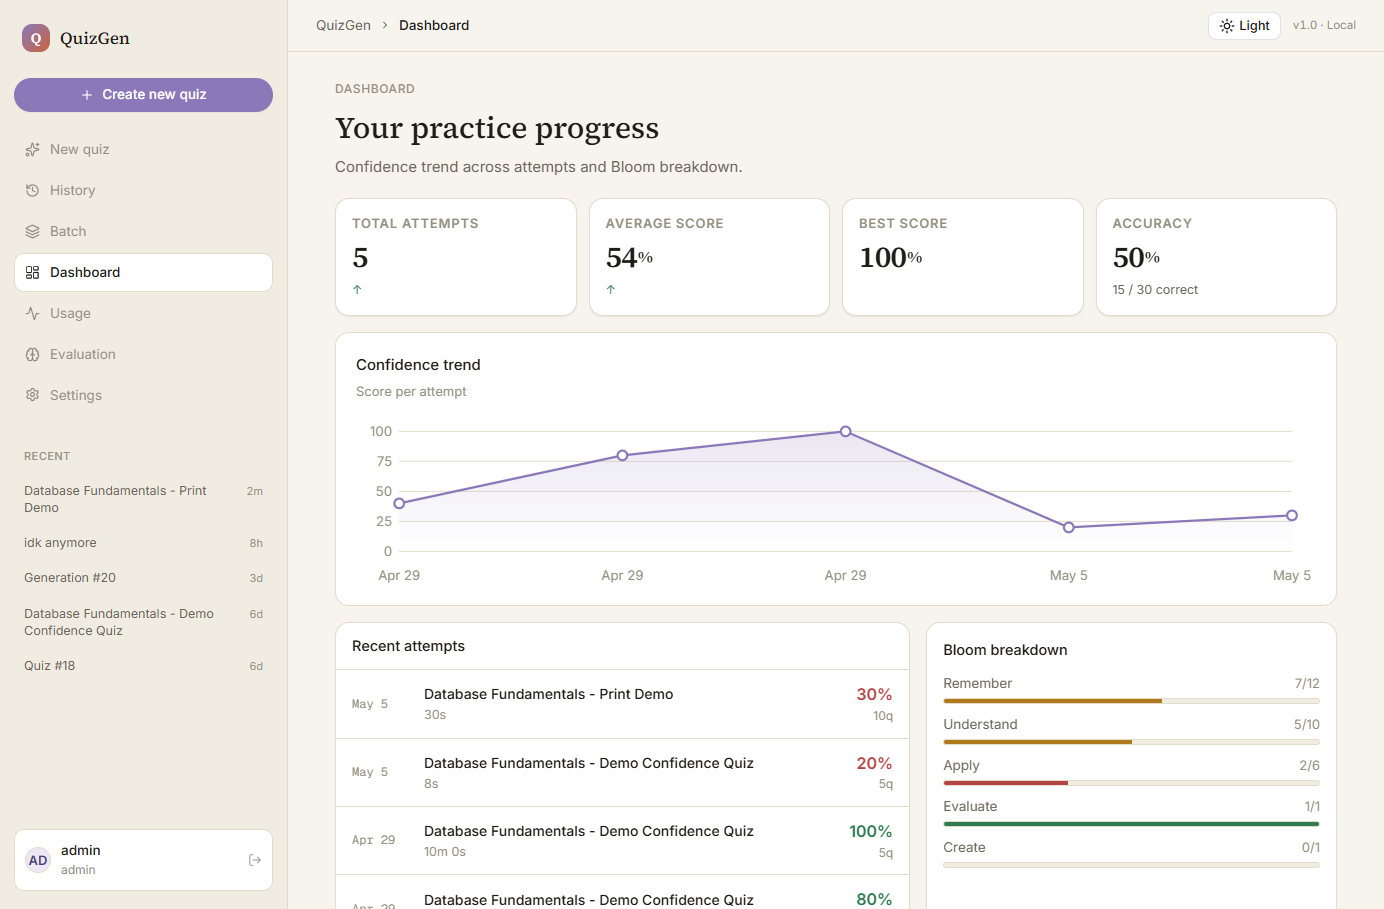
\includegraphics[width=0.95\linewidth]{08-dashboard-confidence-trend.png}
  \caption{Dashboard showing attempt score trend and topic-based practice
           review from stored quiz attempts.}
  \label{fig:confidence-trend}
\end{figure}

The usage dashboard records provider-level API information. It shows token
consumption, generation count, provider breakdown, recent calls, and
fallback events. I used this page during testing to see when generation
moved from Groq to a fallback provider. This mattered because quota and
provider availability affected several test runs.

\begin{figure}[H]
  \centering
  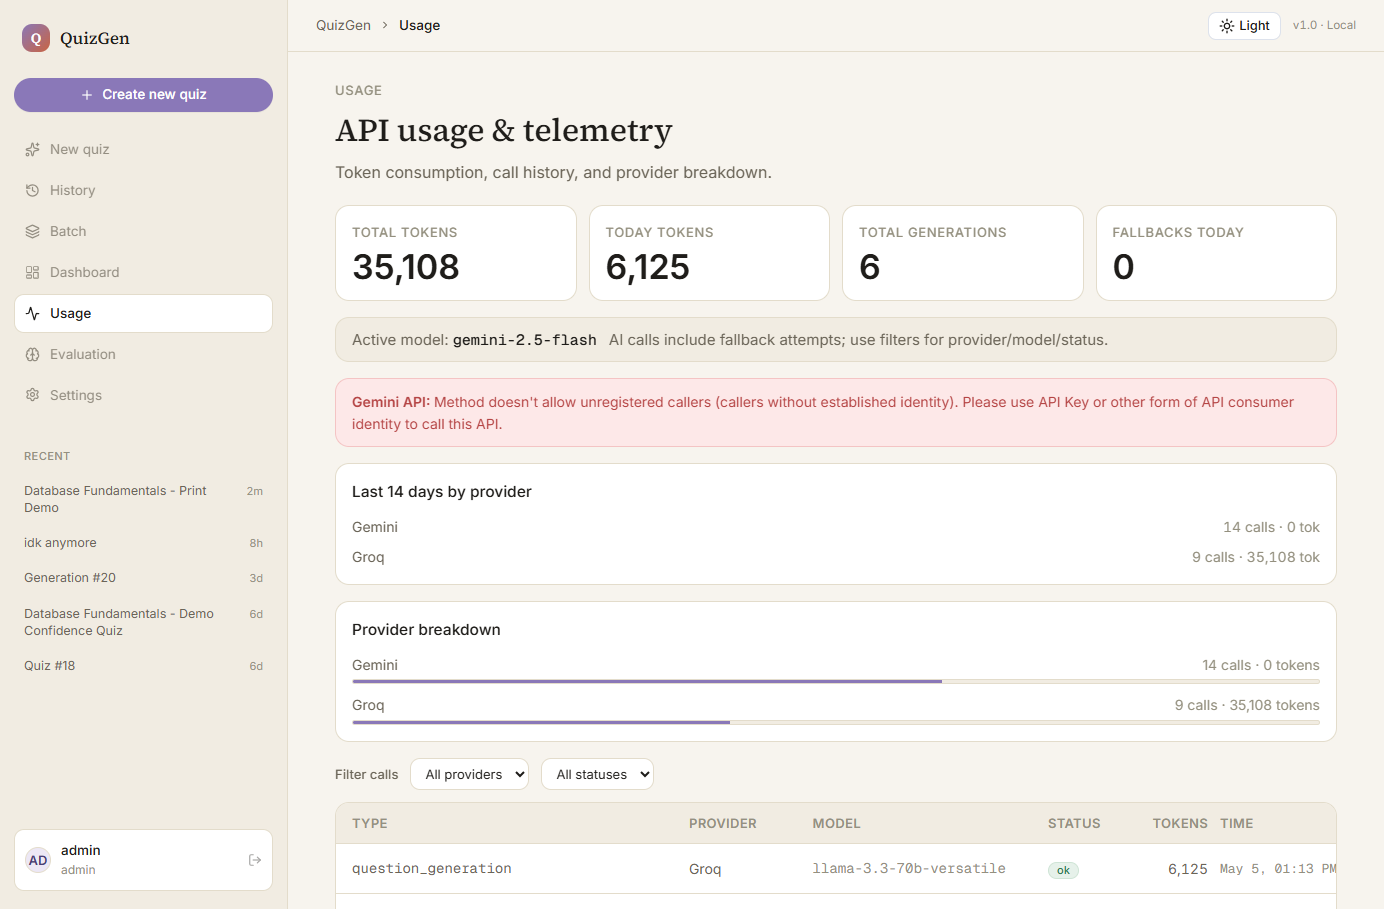
\includegraphics[width=0.95\linewidth]{10-usage-dashboard.png}
  \caption{Usage dashboard showing per-provider API call statistics and
           token consumption.}
  \label{fig:usage-dashboard}
\end{figure}

\subsection{Testing and Demonstration Readiness}

I checked the final implementation with frontend linting, frontend
production build, backend Python compilation, API health checks, route
rendering, and manual workflow testing. The goal was not to prove production
reliability. The goal was to verify that the thesis demo could run from
document upload to quiz attempt and that common failure cases had visible
handling.

Table~\ref{tab:test-summary} summarizes the smoke-test evidence. I captured
the final screenshot set on 5 May 2026 in light mode because the printed
thesis needs readable text, charts, and UI labels.

\begin{table}[H]
  \centering
  \singlespacing
  \caption{Implementation smoke-test summary.}
  \label{tab:test-summary}
  \small
  \begin{tabular}{@{}p{3.3cm}p{1.8cm}p{8.3cm}@{}}
    \toprule
    \textbf{Area} & \textbf{Result} & \textbf{Evidence} \\
    \midrule
    Frontend lint & Pass & \texttt{npm run lint} completed successfully \\
    Frontend production build & Pass & Next.js build passed outside the Windows sandbox \\
    Backend Python compile & Pass & \texttt{compileall} completed for backend modules \\
    Backend health & Pass & \texttt{/api/health} returned \texttt{\{"status":"ok"\}} \\
    Auth and protected routing & Pass & Admin login, logout, and protected redirect checked \\
    Frontend workflow smoke & Pass & Source, Pattern, Generate, Review, Quiz, Attempt, History, Dashboard, Usage, Evaluation, Settings, and Batch checked \\
    Live AI/key smoke & Pass & One demo generation completed and was submitted as a quiz attempt \\
    Full evaluation rerun & Cached & Thesis uses the saved 2026-05-04 evaluation artifacts \\
    \bottomrule
  \end{tabular}
\end{table}

The browser smoke test covered authentication, protected redirects, document
selection, long filename display, pattern selection, generation, review
rename and export controls, quiz practice, attempt review, History,
Dashboard, Usage, Evaluation, Settings, and Batch. One issue still remains
in the dashboard trend aggregation. The chart does not yet provide a clean
per-quiz analytics view, so I report it as a limitation instead of
presenting it as a finished production feature.

The implementation still demonstrates the complete research workflow:
document upload, pattern configuration, MCQ generation, grounding review,
quiz practice, attempt review, dashboard visualization, usage monitoring,
and evaluation reporting. Remaining engineering issues are recorded as
limitations and future work.

\clearpage
\section{Discussion and Evaluation}

\subsection{Evaluation Design}

In my evaluation, I wanted to check whether the added pipeline components
actually help, not only whether the LLM can write fluent questions. I used
four documents, ten topics, three repeated runs per baseline, and six
questions per topic. The comparison focuses on three configurations:
vanilla generation, RAG-only generation, and the full system with pattern
conditioning. Table~\ref{tab:eval-setup} summarises the evaluation
configuration.

\begin{table}[H]
  \centering
  \singlespacing
  \caption{Evaluation setup.}
  \label{tab:eval-setup}
  \small
  \begin{tabular}{@{}p{3.2cm}p{10.2cm}@{}}
    \toprule
    \textbf{Parameter} & \textbf{Value} \\
    \midrule
    Documents           & 4 (IT Fundamentals, DB Fundamentals, OS Principles, Network Security) \\
    Topics              & 10 (7 English, 3 Vietnamese) \\
    Questions per topic & 6 \\
    Repeats per baseline & 3 \\
    Total question sets  & 90 (3 baselines $\times$ 10 topics $\times$ 3 repeats) \\
    Generation model    & \textit{meta-llama/llama-4-scout-17b-16e-instruct} via Groq \\
    Judge model         & Core run: \textit{gemini-2.5-flash}; post-review ablation: OpenRouter auto-free \\
    Embedding model     & Core run: \textit{gemini-embedding-001}; post-review ablation: OpenRouter embedding model \\
    Retrieval top-$k$   & 3 (RAG only and full system); 1 (vanilla) \\
    Prompt version      & v1 \\
    Random seed         & 42 \\
    \bottomrule
  \end{tabular}
\end{table}

The evaluator is configured through \texttt{eval/config.yaml}. Some model
resolution still depends on environment variables and router fallback, so I
treat the saved result files as part of the evidence. In particular,
\texttt{runs.csv} and \texttt{history.md} are append-only records, while
\texttt{comparison.csv}, \texttt{details.csv}, and
\texttt{failure\_analysis.md} describe the latest run snapshot.

The three core baselines are separated by what they remove. Baseline
vanilla removes retrieval and pattern conditioning. RAG only adds top-$k=3$
semantic retrieval but keeps pattern conditioning out. The full system uses
retrieval, pattern examples, and Bloom distribution control. All three use
the same generation model,
\textit{meta-llama/llama-4-scout-17b-16e-instruct}, so the result is about
the pipeline design rather than model strength.

After advisor feedback, I also ran a smaller retrieval ablation on the full
system. This ablation compares dense retrieval, hybrid dense+BM25 retrieval,
and hybrid retrieval with LLM reranking. I report it separately because it
answers a narrower question: whether reranking helps inside the already
pattern-aware system.

\subsection{Metrics}

Before defining the metrics, I define what I mean by a useful MCQ set. The
questions should be grounded in the lecture material, follow the requested
Bloom or difficulty plan, have clear answer keys, and avoid repeating the
same concept too much. These requirements cannot be measured by one number,
so I use several metrics.

Table~\ref{tab:metrics} defines the nine metrics computed by the
evaluation pipeline.

\begin{table}[H]
  \centering
  \singlespacing
  \caption{Evaluation metrics, definitions, and desired direction.}
  \label{tab:metrics}
  \begin{tabular}{@{}p{3.1cm}p{1.2cm}p{6.1cm}p{1.2cm}@{}}
    \toprule
    \textbf{Metric} & \textbf{Symbol} & \textbf{Definition} & \textbf{Better} \\
    \midrule
    Recall@$k$ & R@$k$ &
      Fraction of ground-truth chunks present in the top-$k$ retrieved chunks &
      Higher \\
    MRR & MRR &
      Mean reciprocal rank of the first ground-truth chunk in the ranked list &
      Higher \\
    Semantic grounding & SG &
      Mean normalised cosine similarity between each question embedding and the
      source chunk embeddings; range $[0, 1]$ &
      Higher \\
    Bloom KL divergence & KL &
      KL divergence between the target Bloom distribution and the observed
      Bloom label distribution of generated questions; lower means closer
      alignment &
      Lower \\
    LLM judge score & J &
      Mean of four criteria (relevance, correctness, clarity, groundedness)
      scored 1--5 by a \textit{gemini-2.5-flash} judge &
      Higher \\
    Diversity & D &
      1 minus the mean pairwise normalised cosine similarity among question
      embeddings; measures lexical and semantic variety &
      Higher \\
    Topic confusion rate & TC &
      Fraction of generated questions whose embedding aligns more strongly
      with non-target retrieved chunks than expected target chunks &
      Lower \\
    Machine answer correctness & AC &
      Fraction of questions for which an independent verifier selects the
      same answer option as the generated answer key using source context &
      Higher \\
    Questions returned & Q &
      Count of valid questions returned per topic; expected value is 6 &
      $= 6$ \\
    \bottomrule
  \end{tabular}
\end{table}

Recall@$k$ and MRR check retrieval against annotated chunks. Semantic
grounding, Bloom KL divergence, judge score, and diversity check generation
quality from different sides. Questions returned is included because a
system that returns fewer than the requested six questions is not reliable
for the workflow.

Bloom KL uses the requested Bloom or difficulty plan as the target
distribution and the generated \texttt{bloom\_level} labels as the observed
distribution. This metric has a limitation: the same LLM that writes the
question also outputs the Bloom label. If the label is invalid, the backend
maps from difficulty as a fallback. Therefore, Bloom KL should be read as a
distribution-control signal, not as a perfect human-verified Bloom
classification.

Semantic grounding is also a proxy. A high score means the question text is
semantically close to the source, but it does not prove the answer key is
correct. I also report failure analysis and answer-checking signals because
of this gap.

The two post-review metrics were added because of advisor discussion. Topic
confusion checks whether a question drifts toward another topic in the same
document. Machine answer correctness checks whether an independent verifier
chooses the same answer key using the source chunks. These metrics are not
perfect, but they expose failures that the first metric set may hide.

\subsection{Baseline Rationale}

The baselines remove components one by one. Vanilla is the closest to a
manual ChatGPT workflow: give content and ask for MCQs. RAG only adds
source retrieval but does not use exam-pattern examples. The full system
adds both retrieval and pattern/Bloom conditioning. This setup lets me ask
two separate questions: whether retrieval improves grounding, and whether
pattern conditioning improves Bloom alignment.

All baselines use the same generation model. This avoids mixing pipeline
effects with model-strength effects.

\subsection{Quantitative Results}

Table~\ref{tab:results} reports the mean and standard deviation for each
metric across three repeated runs.

\clearpage

\begin{table}[H]
  \centering
  \singlespacing
  \caption{Core baseline comparison (mean $\pm$ std, 3 repeats, 10 topics).}
  \label{tab:results}

  \small
  \setlength{\tabcolsep}{4pt}
  \renewcommand{\arraystretch}{1.08}

  \resizebox{\linewidth}{!}{%
    \begin{tabular}{@{}lrrrrr@{}}
      \toprule
      \textbf{Baseline} &
      \textbf{SG} $\uparrow$ &
      \textbf{KL} $\downarrow$ &
      \textbf{Judge} $\uparrow$ &
      \textbf{Diversity} $\uparrow$ &
      \textbf{Q ret.} \\
      \midrule
      Baseline vanilla
        & $0.7912 \pm 0.0048$
        & $18.029 \pm 1.685$
        & $3.783 \pm 0.095$
        & $0.2152 \pm 0.0033$
        & $6.0 \pm 0.0$ \\
      RAG only
        & $0.9369 \pm 0.0030$
        & $11.636 \pm 0.960$
        & $4.000 \pm 0.000$
        & $0.1711 \pm 0.0031$
        & $6.0 \pm 0.0$ \\
      Full system
        & $0.9334 \pm 0.0021$
        & $3.905 \pm 0.782$
        & $4.075 \pm 0.152$
        & $0.1731 \pm 0.0032$
        & $6.0 \pm 0.0$ \\
      \bottomrule
    \end{tabular}%
  }
\end{table}

Recall@$k$ and MRR were 1.0000 $\pm$ 0.0000 for all three baselines. In
this small golden dataset, the annotated chunk is easy for the retriever to
find. Because of that, these two metrics do not explain the main difference
between baselines. The more useful differences appear in grounding, Bloom
KL, judge score, and answer-checking signals.

Table~\ref{tab:retrieval-ablation} reports the post-review retrieval
ablation from the cached run \texttt{2026-05-04T14:42:34Z}. Unlike
Table~\ref{tab:results}, this table compares only variants of the full
system and should be read as an ablation of retrieval strategy rather than
as a replacement for the core baseline comparison.

\begin{table}[H]
\centering
\singlespacing
\caption{Post-review retrieval ablation for full-system variants.}
\label{tab:retrieval-ablation}

\resizebox{\linewidth}{!}{
\begin{tabular}{@{}lrrrrr@{}}
\toprule
Baseline & SG $\uparrow$ & KL $\downarrow$ & Judge $\uparrow$ & Diversity $\uparrow$ & Q ret. \\
\midrule
Baseline vanilla & 0.7912 $\pm$ 0.0048 & 18.029 $\pm$ 1.685 & 3.783 $\pm$ 0.095 & 0.2152 $\pm$ 0.0033 & 6.0 $\pm$ 0.0 \\
RAG only & 0.9369 $\pm$ 0.0030 & 11.636 $\pm$ 0.960 & 4.000 $\pm$ 0.000 & 0.1711 $\pm$ 0.0031 & 6.0 $\pm$ 0.0 \\
Full system & 0.9334 $\pm$ 0.0021 & 3.905 $\pm$ 0.782 & 4.075 $\pm$ 0.152 & 0.1731 $\pm$ 0.0032 & 6.0 $\pm$ 0.0 \\
\bottomrule
\end{tabular}
}
\end{table}

The ablation result is mixed. Hybrid retrieval slightly improves semantic
grounding and Bloom KL compared with dense retrieval, which suggests that
exact keyword evidence can help dense semantic matching. The reranked
variant gives a better topic-confusion value and a higher judge score, but
its machine answer-correctness value drops from 0.9944 to 0.9444. For this
reason, I treat reranking as a useful diagnostic direction, not as a solved
default setting.

\textbf{Semantic grounding.} RAG changes the grounding score most clearly.
Vanilla generation reaches 0.7912, while RAG only reaches 0.9369. The
reason is straightforward: the model gets smaller and more relevant source
chunks instead of relying on its internal knowledge. The full system scores slightly lower at 0.9334 because pattern
conditioning asks the model to rephrase source material into exam-style
stems and distractors — intentionally moving the text away from raw source
embeddings.

\textbf{Bloom KL divergence.} The full system has the strongest Bloom
alignment result. KL falls from 18.029 in vanilla to 3.905 in the full
system. RAG only improves the value to 11.636, but the main drop happens
after pattern and Bloom instructions are added.

\textbf{LLM judge score.} The full system also has the highest judge score,
4.075. The difference over RAG only is small, but it is consistent with the
idea that pattern examples improve the structure of the questions, not only
their source relevance.

\textbf{Diversity.} RAG methods produce lower semantic diversity than
vanilla prompting. That is expected here: quiz generation wants focus.
Questions should stay anchored to the selected topic, not scatter across
semantic space. Lower diversity looks bad in creative writing but is the
right behavior for lecture-grounded MCQs.

\subsection{Practical Interpretation of Results}

The results match how I expected the pipeline to behave. Retrieval mainly
controls \textit{what} the model asks about. Pattern and Bloom instructions
mainly control \textit{how} the model asks. This separation is important:
RAG alone gives source relevance, but it does not fully control cognitive
level.

The full system has slightly lower semantic grounding than RAG only
(0.9334 versus 0.9369). The 0.4\% drop is a known trade-off: pattern
conditioning improves Bloom KL divergence from 11.636 to 3.905 and raises
the judge score, both more important for educational use than raw semantic
closeness to the source chunks.


\subsection{Failure Analysis}

The failure analysis looks at cases that still failed after generation. I
flagged a topic-level case when Bloom KL was above 8 or when the judge score
was below 4. Table~\ref{tab:failures} presents representative cases.

\begin{table}[H]
  \centering
  \singlespacing
  \caption{Representative failure cases from the evaluation.}
  \label{tab:failures}
  \small
  \begin{tabular}{@{}p{2.8cm}p{2.6cm}p{2.8cm}p{3.2cm}r@{}}
    \toprule
    \textbf{Baseline} & \textbf{Document} & \textbf{Topic} &
    \textbf{Trigger} & \textbf{Value} \\
    \midrule
    Baseline vanilla & os\_basics         & cpu\_scheduling   & Bloom mismatch   & 27.020 \\
    Baseline vanilla & it\_intro          & cloud\_models     & Bloom mismatch   & 26.958 \\
    Baseline vanilla & db\_fundamentals   & acid\_transactions & Low judge score  & 3.500  \\
    RAG only         & os\_basics         & cpu\_scheduling   & Bloom mismatch   & 27.020 \\
    Full system      & db\_fundamentals   & acid\_transactions & Bloom mismatch   & 13.469 \\
    \bottomrule
  \end{tabular}
\end{table}

The failures show three useful patterns. First, Bloom mismatch is the
largest problem in the vanilla baseline. When the target topic needs
\textit{apply} or \textit{analyze} questions, the model often falls back to
definition-style questions. Second, RAG only improves grounding and judge
score, but it cannot decide the cognitive level by itself. Third, the full
system reduces the number of failure-triggering cases, but it still has
difficult topics such as \textit{acid\_transactions} and
\textit{cpu\_scheduling}. These topics were difficult because they require
more than recognizing a definition. A good question needs the model to
preserve constraints such as transaction isolation properties or scheduling
algorithm behavior, and small wording changes in the stem or options can
make the answer key less reliable. These cases show the boundary of
prompt-based Bloom control.

The post-review analysis adds topic confusion and answer mismatch. Topic
confusion showed up even when retrieval recall was perfect. Getting the
right chunk does not guarantee the generated question stays on that topic.
The reranking ablation improved some relevance signals but dropped machine
answer correctness. The trade-off was not worth it, so I am not pushing
reranking as a win.

\subsection{Comparison with Related Work}

Table~\ref{tab:related-comparison} compares QuizGen with the systems from
Chapter~II using evidence that is reported in the papers or in this thesis.
I use this table to show what QuizGen evaluates, not only what features it
claims to have.

\begin{table}[H]
  \centering
  \singlespacing
  \caption{Evidence-based comparison of QuizGen with related systems.}
  \label{tab:related-comparison}
  \begin{tabular}{@{}p{3.2cm}p{2.2cm}p{2.2cm}p{2.2cm}p{2.2cm}@{}}
    \toprule
    \textbf{System} &
    \textbf{Grounding metric reported} &
    \textbf{Bloom alignment evaluated} &
    \textbf{Quiz practice workflow} &
    \textbf{Performance analytics} \\
    \midrule
    Generic ChatGPT         & No & No & No & No \\
    E-QGen \cite{eqgen2024} & No & No & No & No \\
    BUE AQG \cite{bueaqg2024} & User study (80\% satisfaction) & No & No & No \\
    COLING 2025 \cite{coling2025mcq} & BLEU/ROUGE only & No & No & No \\
    \textbf{QuizGen (this thesis)} &
      \textbf{Semantic grounding score (0.93)} &
      \textbf{Bloom KL divergence (3.91)} &
      \textbf{Yes (attempt tracking)} &
      \textbf{Yes (confidence trend)} \\
    \bottomrule
  \end{tabular}
\end{table}

Compared with generic prompting, QuizGen adds retrieval and grounding
review. Compared with RAG-only generation, it adds pattern conditioning and
Bloom control. Compared with static question generation tools, it also adds
practice attempts, history, and dashboard views.

\subsection{Practical Implications for Lecturers and Students}

For lecturers, the takeaway is that QuizGen is a drafting tool, not a final
authoring tool. It can reduce the time spent writing stems and options, and
the grounding status helps identify questions that need closer checking. But
a high grounding score does not mean the answer key is correct, and a valid
Bloom label does not mean the distractor set is fair. The review step is
not optional.

For students, the value is different. The generated questions become timed
practice attempts with explanations, scores, history, and topic-level
feedback. The 80/20 principle applies here: if a student can identify the
two or three weak topics from the dashboard and then practice those
specifically using \texttt{topic\_focus}, the preparation time becomes more
focused than reviewing everything at equal depth.

Generation alone does not make questions useful. The review and
practice workflow around it — grounding check, quiz attempt, explanation,
progress tracking — is what turns generated text into study material. Questions in a text file have no feedback loop. Connected to
attempts, explanations, and progress tracking, the same questions become
usable study material.

\subsection{Threats to Validity}

The evaluation has clear boundaries. Ten topics across four documents means
these results are thesis-scale, not generalizable to all courses. The judge
model has its own biases — it scores based on its training, not on a
lecturer's real expectations. The grounding score is cosine similarity; it
shows whether the question text is near the source chunks, but says nothing
about whether the answer key is right.

Retrieval metrics maxed out here. Recall@$k$ and MRR hit 1.0 because the
annotated chunks are easy targets in a small document set. A larger, noisier
collection would likely show more variance. The evaluation also ran on one
model in a local single-user prototype. A classroom deployment with real
concurrent users and more diverse materials would need a separate round of
testing.

\subsection{Summary of Findings}

The evaluation gives three main findings. First, RAG improves semantic
grounding from 0.7912 to 0.9369. Second, pattern conditioning reduces Bloom
KL from 11.636 to 3.905 when added on top of RAG. Third, the full system has
the best judge score, 4.075, while still returning all requested questions.
The remaining weakness is individual-topic Bloom control, especially for
higher-order questions. Lecturer review is still necessary.

\clearpage
\section{Conclusion and Future Work}

\subsection{Conclusion}

When I started this project, the study workflow I used was already working
in a rough way: look at old exam questions, ask an LLM to make more, and
check the answers manually. What was missing was any way to know whether the
questions actually came from the lecture material, whether the style matched
the exam, and whether practice results were improving over time. QuizGen is
the answer to all three of those gaps in one place.

The implementation covers the full path from lecture material to student
practice. PDF, DOCX, and PPTX files are split into word-level chunks,
embedded, and searched at generation time. Retrieved chunks and optional
pattern examples go into the prompt. The backend parses structured MCQ
output, stores the generation, and supports quiz attempts, attempt review,
history, and dashboard views. The scope is a thesis prototype, but the workflow goes end-to-end:
upload, generation, review, quiz practice, attempt history, and dashboard.

The evaluation confirmed that the added pipeline components help in
measurable ways. RAG improved semantic grounding from 0.7912 to 0.9369.
Adding pattern and Bloom conditioning on top of RAG reduced Bloom KL from
11.636 to 3.905. The full system also reached the highest judge score,
4.075, while still returning all requested questions. The remaining
weakness is that some topics, especially those requiring higher-order
questions, still produce Bloom mismatches. Lecturer review is still
necessary, and I designed the review step into the workflow from the start.

\subsection{Contributions}

Here is what I actually built and what I consider the contributions of this
work:

\begin{enumerate}
  \item I implemented a pattern-aware RAG pipeline that uses semantic
        retrieval, sample exam questions, and Bloom distribution settings
        to guide MCQ generation without fine-tuning a model.
  \item I designed a grounding proxy based on normalized cosine similarity
        between generated question content and the source material, and
        extended it with topic-confusion and answer-key verification signals.
        These are review aids, not replacements for lecturer judgment.
  \item I built the full web workflow around the pipeline: document upload,
        generation, review, quiz practice, attempt review, history, usage
        tracking, topic mastery review, focused topic practice, and
        dashboard views.
  \item I set up a reproducible evaluation with fixed baselines, repeated
        runs, structured result files, checkpoint logs, failure analysis, and
        a post-review retrieval ablation comparing dense retrieval, hybrid
        retrieval, and hybrid retrieval with reranking.
  \item I added provider routing for Groq, Gemini, OpenRouter, and local
        Ollama fallback, together with usage and token logging so that
        development could continue when one provider was rate-limited.
\end{enumerate}

\subsection{Achievement of Objectives}

Table~\ref{tab:objective-achievement} summarizes how the implementation and
evaluation address the objectives introduced in Chapter~I.

\begin{table}[H]
  \centering
  \singlespacing
  \caption{Achievement of thesis objectives.}
  \label{tab:objective-achievement}
  \begin{tabular}{@{}p{5.0cm}p{7.0cm}@{}}
    \toprule
    \textbf{Objective} & \textbf{Achievement in QuizGen} \\
    \midrule
    Process PDF, DOCX, and PPTX lecture materials &
    Implemented document upload, extraction, chunking, and storage through
    the document processor service. \\
    Apply retrieval-augmented generation &
    Implemented embedding generation, cosine-similarity chunk retrieval,
    prompt context injection, and post-review hybrid/rerank ablation modes. \\
    Incorporate exam-pattern conditioning &
    Implemented pattern creation, pattern storage, and few-shot prompt
    injection during generation. \\
    Generate structured MCQ outputs &
    Implemented JSON-based question generation with answer options, correct
    answers, explanations, difficulty labels, and Bloom labels. \\
    Provide grounding evaluation &
    Implemented semantic grounding scores, topic-confusion analysis,
    answer-key verification, and review-facing grounding status labels. \\
    Implement quiz practice and analytics &
    Implemented quiz attempt submission, attempt review, confidence trend,
    Bloom breakdown, topic mastery review, focused topic practice, history,
    and usage dashboards. \\
    Evaluate against baselines &
    Implemented a reproducible evaluation runner and reported vanilla,
    RAG-only, full-system, and post-review retrieval-ablation comparisons. \\
    \bottomrule
  \end{tabular}
\end{table}

At prototype scale, the objectives were achieved. The system can upload
materials, generate questions, review grounding, run quizzes, store
attempts, and show dashboard information. The evaluation also shows
measurable improvement from retrieval and pattern conditioning. Production
readiness and fully automated exam authoring remain outside the scope.

\subsection{Limitations}
\label{sec:limitations}

The main limitations are practical. QuizGen currently focuses on MCQs only.
The evaluation dataset has ten topics across four documents, so it is not
large enough for a broad domain claim. The system was tested locally, not in
a real class with many concurrent users. The grounding score is a semantic
proxy and cannot prove factual correctness. The answer verifier helps, but
it also cannot replace lecturer checking.

There are also implementation limits. The current generation API is still
single-document. The batch workflow can accept multiple document ids, but it
creates independent quizzes per document rather than one merged quiz with a
controlled split. The backend uses SQLite and a single FastAPI process,
which is acceptable for thesis-scale testing but not for production
deployment.

\subsection{Future Work}
\label{subsec:future}

The next improvement should be true multi-document retrieval. A real course
often has slides, notes, and textbook sections together. The system should
retrieve across those files and control how much content comes from each
source. Retrieval can also use headings, slide numbers, and better keyword
expansion. Reranking should be studied more, but only after answer
correctness is checked more strongly.

Generation also needs better control. Future work should check whether the
difficulty label really matches the cognitive demand of each question. It
should also support safer pattern variation, such as same-form questions,
changed-number questions, fill-in-the-blank variants, and tricky
distractors. These features need stronger answer verification because small
changes can easily make the answer wrong.

The evaluation should be expanded with more subjects, more document types,
more languages, and human lecturer review. Lecturer review is especially
important for distractor quality and pedagogical usefulness. On the
deployment side, the system should move beyond SQLite, add asynchronous
generation jobs, improve role-based access control, support PDF export and
spaced repetition, and test local LLM fallback more formally.

For student practice, the most useful future feature is per-topic
performance tracking. If each generated question is linked to a source
section or topic tag, the dashboard can show which topics a student is weak
at. The system could then generate a new remedial quiz from those weak
topics. This would make QuizGen closer to an adaptive study tool instead of
only a question generator.

% ════════════════════════════════════════════════════════════════════════════
%  REFERENCES
% ════════════════════════════════════════════════════════════════════════════

\newpage
\addcontentsline{toc}{section}{List of References}
\renewcommand{\refname}{LIST OF REFERENCES}

\begin{thebibliography}{99}
\setlength{\itemsep}{0.5\baselineskip}

\bibitem{brown2020gpt3}
Brown, T. B., Mann, B., Ryder, N., Subbiah, M., Kaplan, J., Dhariwal, P.,
Neelakantan, A., Shyam, P., Sastry, G., Askell, A., Agarwal, S.,
Herbert-Voss, A., Krueger, G., Henighan, T., Child, R., Ramesh, A.,
Ziegler, D. M., Wu, J., Winter, C., Hesse, C., Chen, M., Sigler, E.,
Litwin, M., Gray, S., Chess, B., Clark, J., Berner, C., McCandlish, S.,
Radford, A., Sutskever, I., and Amodei, D. 2020. Language models are
few-shot learners. \textit{Advances in Neural Information Processing
Systems}, 33, 1877--1901.

\bibitem{xu2024survey1}
Xu, X., Gan, Y., Zhang, X., Shi, Y., Li, Y., Dong, Y., and Tang, J. 2024.
Large language models for education: A survey and outlook.
\textit{arXiv preprint arXiv:2403.18105}.

\bibitem{xu2024survey2}
Xu, X., Li, Y., Dong, Y., Zhang, X., Shi, Y., Gan, Y., and Tang, J. 2024.
Large language models for education: A survey.
\textit{arXiv preprint arXiv:2405.13001}.

\bibitem{frontiers2024chatgpt}
Rasul, T., Nair, S., Kalendra, D., Robin, M., de Oliveira Santini, F.,
Ladeira, W. J., Sun, M., Day, I., Rather, R. A., and Heathcote, L. 2024.
The role of ChatGPT in higher education: Benefits, challenges, and future
research directions. \textit{Frontiers in Education}, 8, 1--15.

\bibitem{ieeebigdata2023}
Pham, A., Dobbins, C., and Ning, H. 2023. Evaluating ChatGPT for question
generation from passage context. In \textit{Proceedings of the IEEE
International Conference on Big Data (BigData)}, pp. 4105--4113. IEEE.

\bibitem{danyaro2024hallucination}
Danyaro, K. U., Liew, M. S., Ahmed, A., and Hussain, A. 2024.
Hallucinations in large language models for education: Challenges and
mitigation. \textit{International Journal of Technology in Learning
and Education}.

\bibitem{lewis2020rag}
Lewis, P., Perez, E., Piktus, A., Petroni, F., Karpukhin, V., Goyal, N.,
K\"{u}ttler, H., Lewis, M., Yih, W., Rockt\"{a}schel, T., Riedel, S., and
Kiela, D. 2020. Retrieval-augmented generation for knowledge-intensive NLP
tasks. \textit{Advances in Neural Information Processing Systems}, 33,
9459--9474.

\bibitem{es2023ragas}
Es, S., James, J., Anke, L. E., and Schockaert, S. 2023.
RAGAS: Automated evaluation of retrieval augmented generation.
\textit{arXiv preprint arXiv:2309.15217}.

\bibitem{white2023prompt}
White, J., Fu, Q., Hays, S., Sandborn, M., Olea, C., Gilbert, H.,
Elnashar, A., Spencer-Smith, J., and Schmidt, D. C. 2023.
A prompt pattern catalog to enhance prompt engineering with ChatGPT.
\textit{arXiv preprint arXiv:2302.11382}.

\bibitem{weng2023prompteng}
Weng, L. 2023. Prompt engineering.
\textit{Lil'Log blog}. [Online]. Available:
\url{https://lilianweng.github.io/posts/2023-03-15-prompt-engineering/}.
[Accessed: May 1, 2026].

\bibitem{bloom1956taxonomy}
Bloom, B. S., Engelhart, M. D., Furst, E. J., Hill, W. H., and
Krathwohl, D. R. 1956. \textit{Taxonomy of Educational Objectives:
The Classification of Educational Goals. Handbook I: Cognitive Domain}.
David McKay, New York.

\bibitem{anderson2001taxonomy}
Anderson, L. W., Krathwohl, D. R., Airasian, P. W., Cruikshank, K. A.,
Mayer, R. E., Pintrich, P. R., Raths, J., and Wittrock, M. C. 2001.
\textit{A Taxonomy for Learning, Teaching, and Assessing: A Revision of
Bloom's Taxonomy of Educational Objectives}. Longman, New York.

\bibitem{anderson1985its}
Anderson, J. R., Boyle, C. F., and Reiser, B. J. 1985.
Intelligent tutoring systems. \textit{Science}, 228(4698), 456--462.

\bibitem{springer2022aes}
Springer Nature. 2022. Automated essay scoring systems. In
\textit{Encyclopedia of Education and Information Technologies}.
[Online]. Available:
\url{https://link.springer.com/rwe/10.1007/978-981-19-2080-6_59}.
[Accessed: May 1, 2026].

\bibitem{khanmigo2026}
Khan Academy. \textit{Khanmigo: Khan Academy's AI-powered teaching
assistant and tutor}. [Online]. Available:
\url{https://www.khanmigo.ai/}. [Accessed: May 1, 2026].

\bibitem{duolingo2023max}
Duolingo Team. 2023. Introducing Duolingo Max, a learning experience
powered by GPT-4. [Online]. Available:
\url{https://blog.duolingo.com/duolingo-max/}. [Accessed: May 1, 2026].

\bibitem{robertson2009bm25}
Robertson, S., and Zaragoza, H. 2009. The probabilistic relevance
framework: BM25 and beyond. \textit{Foundations and Trends in Information
Retrieval}, 3(4), 333--389.

\bibitem{karpukhin2020dpr}
Karpukhin, V., Oguz, B., Min, S., Lewis, P., Wu, L., Edunov, S.,
Chen, D., and Yih, W. 2020. Dense passage retrieval for open-domain
question answering. In \textit{Proceedings of EMNLP 2020}, pp. 6769--6781.

\bibitem{cormack2009rrf}
Cormack, G. V., Clarke, C. L. A., and Buettcher, S. 2009. Reciprocal rank
fusion outperforms Condorcet and individual rank learning methods. In
\textit{Proceedings of SIGIR 2009}, pp. 758--759.

\bibitem{nogueira2019bert}
Nogueira, R., and Cho, K. 2019. Passage re-ranking with BERT.
\textit{arXiv preprint arXiv:1901.04085}.

\bibitem{izacard2021fid}
Izacard, G., and Grave, E. 2021. Leveraging passage retrieval with
generative models for open domain question answering. In
\textit{Proceedings of EACL 2021}, pp. 874--880.

\bibitem{shi2023replug}
Shi, W., Min, S., Yasunaga, M., Seo, M., James, R., Lewis, M.,
Zettlemoyer, L., and Yih, W. 2023. REPLUG: Retrieval-augmented black-box
language models. \textit{arXiv preprint arXiv:2301.12652}.

\bibitem{saadfalcon2023ares}
Saad-Falcon, J., Khattab, O., Potts, C., and Zaharia, M. 2023.
ARES: An automated evaluation framework for retrieval-augmented generation
systems. \textit{arXiv preprint arXiv:2311.09476}.

\bibitem{pan2019nqg}
Pan, L., Lei, W., Chua, T.-S., and Kan, M.-Y. 2019.
Recent advances in neural question generation.
\textit{arXiv preprint arXiv:1905.08949}.

\bibitem{kurdi2020aqg}
Kurdi, G., Leo, J., Parsia, B., Sattler, U., and Al-Emari, S. 2020.
A systematic review of automatic question generation for educational
purposes. \textit{International Journal of Artificial Intelligence in
Education}, 30, 121--204.

\bibitem{wei2022cot}
Wei, J., Wang, X., Schuurmans, D., Bosma, M., Ichter, B., Xia, F.,
Chi, E., Le, Q. V., and Zhou, D. 2022. Chain-of-thought prompting elicits
reasoning in large language models. In \textit{Advances in Neural
Information Processing Systems}, 35, 24824--24837.

\bibitem{wang2022selfconsistency}
Wang, X., Wei, J., Schuurmans, D., Le, Q. V., Chi, E., Narang, S.,
Chowdhery, A., and Zhou, D. 2022. Self-consistency improves chain of
thought reasoning in language models. \textit{arXiv preprint
arXiv:2203.11171}.

\bibitem{ouyang2022instructgpt}
Ouyang, L., Wu, J., Jiang, X., Almeida, D., Wainwright, C., Mishkin, P.,
Zhang, C., Agarwal, S., Slama, K., Ray, A., Schulman, J., Hilton, J.,
Kelton, F., Miller, L., Simens, M., Askell, A., Welinder, P.,
Christiano, P. F., Leike, J., and Lowe, R. 2022. Training language models
to follow instructions with human feedback. In \textit{Advances in Neural
Information Processing Systems}, 35, 27730--27744.

\bibitem{ieee2025mcqsurvey}
Alkhuzaey, S., Grasso, F., Payne, T. R., and Tamma, V. 2025.
Text-based question generation using transformers and large language models:
A systematic literature review. \textit{IEEE Transactions on Learning
Technologies}, 18, 1--20.

\bibitem{coling2025mcq}
Rodríguez-García, M., Sánchez-Rada, J. F., and Iglesias, C. A. 2025.
Automated MCQ generation and validation using large language models.
In \textit{Proceedings of the 31st International Conference on
Computational Linguistics (COLING 2025)}, pp. 1842--1853.

\bibitem{eqgen2024}
Hadifar, A., Bitew, S. K., Deleu, J., Develder, C., and Demeester, T. 2024.
E-QGen: Educational lecture abstract-based question generation system.
\textit{arXiv preprint arXiv:2404.13547}.

\bibitem{bueaqg2024}
Shaban, W. M., Elhoseny, M., and Hassanien, A. E. 2024.
Automatic question generation using GPT, T5, and BERT for educational
assessment. \textit{Journal of King Saud University -- Computer and
Information Sciences}, 36(3), 101983.

\bibitem{quillionz2026}
Quillionz. \textit{Quillionz: AI-powered question generator}. [Online].
Available: \url{https://quillionz.com/}. [Accessed: May 1, 2026].

\bibitem{questgen2026}
Questgen. \textit{Questgen: AI quiz generator}. [Online]. Available:
\url{https://www.questgen.ai/}. [Accessed: May 1, 2026].

\bibitem{google2026geminiembedding}
Google AI for Developers. \textit{Gemini API embeddings documentation}.
[Online]. Available: \url{https://ai.google.dev/gemini-api/docs/embeddings}.
[Accessed: May 1, 2026].

\end{thebibliography}

% ════════════════════════════════════════════════════════════════════════════
%  APPENDICES
% ════════════════════════════════════════════════════════════════════════════

\newpage
\addcontentsline{toc}{section}{Appendices}

\begin{center}
  \textbf{APPENDICES}
\end{center}

\vspace{1cm}

\section*{Appendix A: Example Generated MCQs}
\addcontentsline{toc}{subsection}{Appendix A: Example Generated MCQs}

The following examples illustrate the structure of a generated question
record. They are not synthetic examples; they are taken from the local
SQLite database \texttt{backend/data/quizgen.db}, generation id 19, titled
\textit{Database Fundamentals - Demo Confidence Quiz}. The generation was
completed on \texttt{2026-04-29T04:10:12.402146+00:00}, used provider
\texttt{groq}, prompt version \texttt{v1}, and recorded token usage of
5{,}246. The generation contains five MCQs.

\begin{enumerate}
  \item \textbf{Question.} What is the main problem with managing data
        resources in a traditional file environment?

        \textbf{Options.} A. Data redundancy and inconsistency; B. Lack of
        data sharing and availability; C. Poor security; D. All of the
        above.

        \textbf{Correct answer.} D. All of the above.

        \textbf{Explanation.} According to the source material, the
        traditional file environment has several problems, including data
        redundancy, data inconsistency, program-data dependence, lack of
        flexibility, poor security, and lack of data sharing and
        availability.

        \textbf{Difficulty and Bloom level.} Easy; Remember.

  \item \textbf{Question.} What is the primary function of a database
        management system (DBMS)?

        \textbf{Options.} A. To provide a user interface for data entry;
        B. To interface between applications and physical data files;
        C. To provide data storage and retrieval; D. To perform data
        analysis and reporting.

        \textbf{Correct answer.} B. To interface between applications and
        physical data files.

        \textbf{Explanation.} The source material states that a DBMS
        interfaces between applications and physical data files, separating
        logical and physical views of data.

        \textbf{Difficulty and Bloom level.} Medium; Understand.

  \item \textbf{Question.} What is the purpose of normalization in database
        design?

        \textbf{Options.} A. To reduce data redundancy and improve data
        integrity; B. To improve data security; C. To increase data storage
        capacity; D. To enhance data retrieval performance.

        \textbf{Correct answer.} A. To reduce data redundancy and improve
        data integrity.

        \textbf{Explanation.} The source material explains that
        normalization is the process of streamlining complex groupings of
        data to minimize redundant data elements and awkward many-to-many
        relationships.

        \textbf{Difficulty and Bloom level.} Medium; Apply.

  \item \textbf{Question.} What is the primary benefit of using a relational
        DBMS?

        \textbf{Options.} A. Improved data security; B. Increased data
        storage capacity; C. Enhanced data retrieval performance;
        D. Ability to represent data as two-dimensional tables.

        \textbf{Correct answer.} D. Ability to represent data as
        two-dimensional tables.

        \textbf{Explanation.} The source material states that a relational
        DBMS represents data as two-dimensional tables, with each table
        containing data on an entity and its attributes.

        \textbf{Difficulty and Bloom level.} Easy; Remember.

  \item \textbf{Question.} What is the purpose of a data warehouse?

        \textbf{Options.} A. To keep both current and past data collected
        from many operational transaction systems; B. To provide data storage and
        retrieval; C. To perform data analysis and reporting; D. To interface
        between applications and physical data files.

        \textbf{Correct answer.} A. To keep both current and past data
        collected from many operational transaction systems.

        \textbf{Explanation.} The source material explains that a data
        warehouse stores current and historical data from many core
        operational transaction systems, consolidating and standardizing
        information for use across the enterprise.

        \textbf{Difficulty and Bloom level.} Medium; Understand.
\end{enumerate}

\section*{Appendix B: Evaluation Configuration}
\addcontentsline{toc}{subsection}{Appendix B: Evaluation Configuration}

The final evaluation configuration is summarized below. The controlled
comparison uses three core baselines, and the post-review ablation compares
three full-system retrieval modes. Both result sets are reported as cached
runs in Chapter~V.

\begin{longtable}{@{}p{4.0cm}p{9.0cm}@{}}
  \caption{Evaluation configuration summary.}
  \label{tab:appendix-eval-config}\\
  \toprule
  \textbf{Item} & \textbf{Value} \\
  \midrule
  Dataset & \texttt{eval/datasets/golden.json} \\
  Documents & IT Fundamentals, DB Fundamentals, OS Principles, Network Security \\
  Topics & 10 topics, including English and Vietnamese topics \\
  Repeats & 3 per baseline \\
  Questions per topic & 6 \\
  Prompt version & \texttt{v1} \\
  Core baselines & \texttt{baseline\_vanilla}, \texttt{baseline\_rag\_only}, \texttt{full\_system} \\
  Retrieval ablation & \texttt{full\_system}, \texttt{full\_system\_hybrid}, \texttt{full\_system\_hybrid\_rerank} \\
  Generation model & \texttt{meta-llama/llama-4-scout-17b-16e-instruct} \\
  Judge and verifier models & Core run: \texttt{gemini-2.5-flash}; post-review ablation: \texttt{openrouter/auto-free} \\
  Embedding model & Core run: \texttt{gemini-embedding-001}; post-review ablation: \texttt{nvidia/llama-nemotron-embed-vl-1b-v2:free} \\
  Random seed & 42 \\
  Output files & Latest snapshots: \texttt{comparison.csv}, \texttt{details.csv}, \texttt{failure\_analysis.md}; history: \texttt{runs.csv}, \texttt{history.md}; checkpoint JSONL files \\
  \bottomrule
\end{longtable}

The core reproduction command is:

\begin{flushleft}
\small
\begin{verbatim}
set PYTHONPATH=backend && python eval/run_eval.py --config eval/config.yaml ^
  --baselines baseline_vanilla baseline_rag_only full_system
\end{verbatim}
\end{flushleft}

The post-review retrieval ablation command is:

\begin{flushleft}
\small
\begin{verbatim}
set PYTHONPATH=backend && python eval/run_eval.py --config eval/config.yaml ^
  --baselines full_system full_system_hybrid full_system_hybrid_rerank
\end{verbatim}
\end{flushleft}

\section*{Appendix C: Failure Analysis Table}
\addcontentsline{toc}{subsection}{Appendix C: Failure Analysis Table}

The failure-analysis report flags topic-level outputs when Bloom KL
divergence exceeds the configured threshold or the LLM judge score falls
below the configured quality threshold. The representative cases in
Table~\ref{tab:appendix-failure} are used to support the discussion in
Chapter~V.

\begin{table}[H]
  \centering
  \singlespacing
  \caption{Representative evaluation failures.}
  \label{tab:appendix-failure}
  \small
  \begin{tabular}{@{}p{2.8cm}p{2.6cm}p{2.8cm}p{3.2cm}r@{}}
    \toprule
    \textbf{Baseline} & \textbf{Document} & \textbf{Topic} &
    \textbf{Trigger} & \textbf{Value} \\
    \midrule
    Baseline vanilla & os\_basics & cpu\_scheduling & Bloom mismatch & 27.020 \\
    Baseline vanilla & it\_intro & cloud\_models & Bloom mismatch & 26.958 \\
    Baseline vanilla & db\_fundamentals & acid\_transactions & Low judge score & 3.500 \\
    RAG only & os\_basics & cpu\_scheduling & Bloom mismatch & 27.020 \\
    Full system & db\_fundamentals & acid\_transactions & Bloom mismatch & 13.469 \\
    \bottomrule
  \end{tabular}
\end{table}

The dominant failure type is Bloom distribution mismatch. This indicates
that the LLM can follow source content while still failing to produce the
requested cognitive-level mix. The full pipeline has fewer failures of this
kind than the simpler baselines, although some mismatch cases still remain.

\section*{Appendix D: API Endpoint List}
\addcontentsline{toc}{subsection}{Appendix D: API Endpoint List}

Table~\ref{tab:appendix-api} lists the main API groups implemented in the
backend.

\begin{longtable}{@{}p{2.7cm}p{4.5cm}p{6.0cm}@{}}
  \caption{Main API endpoint groups.}
  \label{tab:appendix-api}\\
  \toprule
  \textbf{Group} & \textbf{Representative endpoint} & \textbf{Purpose} \\
  \midrule
  Health & \texttt{GET /api/health} & Verify backend availability \\
  Auth & \texttt{POST /api/auth/register} & Register a user account \\
  Auth & \texttt{POST /api/auth/login} & Issue a JWT token \\
  Auth & \texttt{GET /api/auth/me} & Return current authenticated user \\
  Documents & \texttt{POST /api/documents/upload} & Upload and process lecture material \\
  Documents & \texttt{GET /api/documents/} & List user-owned documents \\
  Patterns & \texttt{POST /api/patterns/} & Create an exam pattern \\
  Patterns & \texttt{GET /api/patterns/} & List saved patterns \\
  Generations & \texttt{POST /api/generations/} & Generate questions \\
  Generations & \texttt{GET /api/generations/} & List saved generations \\
  Quiz & \texttt{POST /api/quiz/submit} & Submit quiz answers \\
  Quiz & \texttt{GET /api/quiz/attempts} & List saved attempts \\
  Dashboard & \texttt{GET /api/dashboard/trend} & Return confidence trend data \\
  Usage & \texttt{GET /api/usage/} & Return provider usage statistics \\
  Evaluation & \texttt{GET /api/eval/latest} & Return latest evaluation result \\
  Batch & \texttt{POST /api/batch/} & Start a batch generation job \\
  \bottomrule
\end{longtable}

\section*{Appendix E: Additional Screenshots}
\addcontentsline{toc}{subsection}{Appendix E: Additional Screenshots}

The screenshot assets used in Chapter~IV are stored under
\texttt{doc/screenshots}. They show the implemented Atelier interface and
serve as the visual record for the thesis demonstration. The last capture
set was taken in light mode so the printed pages are easier to read.

{\small
\begin{longtable}{@{}p{5.4cm}p{7.8cm}@{}}
  \caption{Screenshot asset inventory.}
  \label{tab:appendix-screenshots}\\
  \toprule
  \textbf{File} & \textbf{Shown feature} \\
  \midrule
  \path{01-workflow-source.png} & Document upload and source selection \\
  \path{02-workflow-pattern.png} & Pattern and difficulty configuration \\
  \path{03-workflow-generate-title.png} & Quiz title entry before generation \\
  \path{04-workflow-review.png} & Generated question review \\
  \path{05-quiz-practice.png} & Timed quiz practice screen \\
  \path{06-attempt-review.png} & Attempt review with explanations \\
  \path{07-history-rename.png} & Generation history and rename workflow \\
  \path{08-dashboard-confidence-trend.png} & Per-quiz confidence trend chart \\
  \path{09-evaluation-dashboard.png} & Evaluation dashboard \\
  \path{10-usage-dashboard.png} & Provider usage dashboard \\
  \path{11-settings-config.png} & Configuration and fallback settings \\
  \path{12-batch-workflow.png} & Batch generation workflow \\
  \bottomrule
\end{longtable}
}

\section*{Appendix F: Setup and Run Instructions}
\addcontentsline{toc}{subsection}{Appendix F: Setup and Run Instructions}

The application can be started locally on Windows with the provided batch
script:

\begin{verbatim}
start-all.bat
\end{verbatim}

The script starts the backend on \texttt{http://localhost:8000} and the
frontend on \texttt{http://localhost:3000}. After startup, the backend
health endpoint can be checked with:

\begin{verbatim}
GET http://localhost:8000/api/health
\end{verbatim}

For containerized execution, the application can be started with Docker
Compose:

\begin{verbatim}
docker compose up --build
\end{verbatim}

The recommended demo sequence is:

\begin{enumerate}
  \item Log in with a prepared demo account.
  \item Upload or select a lecture document.
  \item Select either no pattern or a saved exam pattern.
  \item Configure question count, language, and difficulty distribution.
  \item Generate a quiz and inspect the review page.
  \item Start the quiz, submit answers, and open the attempt review page.
  \item Open the dashboard to show confidence trend and Bloom breakdown.
  \item Open the usage dashboard to show provider usage and fallback status.
  \item Open the evaluation dashboard to show the cached baseline results.
\end{enumerate}

If live API quota is unavailable during demonstration, the prepared
screenshots, cached evaluation outputs, and saved generation records can be
used to demonstrate the full workflow without relying on a new LLM call.

\end{document}
